\documentclass[a4paper]{article}

% CJK support: prefer ctex, fallback to XeTeX native line breaking
\IfFileExists{ctex.sty}{
  \usepackage[fontset=fandol]{ctex}
}{
  % Fallback for minimal TeX installs (e.g. MacTeX Basic, TeX Live scheme-basic)
  % without ctex/xeCJK. Uses XeTeX's built-in CJK line breaking.
  \usepackage{fontspec}
  \XeTeXlinebreaklocale "zh"
  \XeTeXlinebreakskip = 0pt plus 1pt
  \IfFontExistsTF{Songti SC}{\setmainfont{Songti SC}}{%
    \IfFontExistsTF{Noto Serif CJK SC}{\setmainfont{Noto Serif CJK SC}}{}%
  }
  \IfFontExistsTF{Heiti SC}{\setsansfont{Heiti SC}}{%
    \IfFontExistsTF{Noto Sans CJK SC}{\setsansfont{Noto Sans CJK SC}}{}%
  }
}

% Basic packages
\usepackage{amsmath, amssymb}
\usepackage{graphicx}
\usepackage[margin=2.5cm]{geometry}
\usepackage[most]{tcolorbox}
\usepackage{etoolbox}
\usepackage{listings}
\usepackage{hyperref}
\usepackage{booktabs}
\usepackage{array}
\usepackage{subcaption}
\usepackage{float}
\usepackage{tikz}
\IfFileExists{pgfplots.sty}{
    \usepackage{pgfplots}
    \pgfplotsset{compat=1.18}
}{}

% ===== Highlight boxes =====
\newtcolorbox{knowledgebox}[1]{
    enhanced, breakable, colback=blue!5!white, colframe=blue!75!black, colbacktitle=blue!75!black,
    coltitle=white, fonttitle=\bfseries, title=#1, attach boxed title to top left={yshift=-2mm, xshift=2mm},
    boxrule=1pt, sharp corners
}

\newtcolorbox{importantbox}[1]{
    enhanced, breakable, colback=yellow!10!white, colframe=yellow!80!black, colbacktitle=yellow!80!black,
    coltitle=black, fonttitle=\bfseries, title=#1, sharp corners
}

\newtcolorbox{warningbox}[1]{
    enhanced, breakable, colback=red!5!white, colframe=red!75!black, colbacktitle=red!75!black,
    coltitle=white, fonttitle=\bfseries, title=#1, sharp corners
}

% ===== Code listings =====
\lstset{
    basicstyle=\ttfamily\small,
    keywordstyle=\color{blue},
    stringstyle=\color{red!60!black},
    commentstyle=\color{green!60!black},
    breaklines=true,
    frame=single,
    numbers=left,
    numberstyle=\tiny\color{gray},
    captionpos=b,
    extendedchars=false
}

% ===== Figure provenance and unit macros =====
% \vtag goes inside \caption{...}; \srcnote{MM:SS--MM:SS} follows the figure environment.
\newcommand{\vtag}{\protect\footnotemark}
\newcommand{\srcnote}[1]{\footnotetext{视频画面时间区间：#1。若为裁剪图，时间区间仍对应原视频画面。}}
% Units work in text and math mode; never hand-write $^\circ$ or \AA inside \mathrm.
\newcommand{\degC}{\ensuremath{^{\circ}\mathrm{C}}}
\newcommand{\um}{\ensuremath{\mu\mathrm{m}}}
\newcommand{\nm}{\ensuremath{\mathrm{nm}}}
\newcommand{\angstrom}{\ensuremath{\text{\AA}}}

% ===== Front-page metadata =====
\newcommand{\notetitle}{人类世初末的青年研究者指南}
\newcommand{\notesubtitle}{Advice for a (Young) Investigator in the First and Last Days of the Anthropocene}
\newcommand{\noteauthors}{主讲：Jascha Sohl-Dickstein（Anthropic）\quad 整理：lecture-to-notes}
\newcommand{\notedate}{2026 年 10 月}
\newcommand{\videochannel}{Jascha Sohl-Dickstein（斯坦福大学 HAI 研讨会 / X @ecommartinez）}
\newcommand{\videopublishdate}{2026-04-18}
\newcommand{\videoduration}{44 分 35 秒（2675 秒）}
\newcommand{\videourl}{https://x.com/ecommartinez/status/2111755238327628202/video/1}
\newcommand{\videocoverpath}{cover.jpg}

\begin{document}

% ===== Title page =====
\begin{titlepage}
\centering
{\Large 课程笔记\par}
\vspace{1.2cm}
{\huge\bfseries \notetitle\par}
\ifdefempty{\notesubtitle}{}{
\vspace{0.3cm}
{\large \notesubtitle\par}
}
\vspace{0.5cm}
{\large \noteauthors\par}
\vspace{0.3cm}
{\large \notedate\par}
\vspace{1.0cm}

\ifdefempty{\videocoverpath}{
{\small 请在生成笔记时填入视频封面图的本地路径。\par}
}{
\includegraphics[width=0.82\textwidth,height=0.40\textheight,keepaspectratio]{\videocoverpath}\par
}

\vfill
\begin{tcolorbox}[width=0.9\textwidth, colback=black!2!white, colframe=black!60, sharp corners]
\textbf{视频作者/频道}：\videochannel\par
\textbf{发布日期}：\videopublishdate\par
\textbf{视频时长}：\videoduration\par
\textbf{视频链接}：
\ifdefempty{\videourl}{
未填写
}{
\href{\videourl}{\nolinkurl{\videourl}}
}
\end{tcolorbox}
\end{titlepage}

\tableofcontents
\newpage

%% --- 正文内容开始 --- %%

\section{引言：站在指数悬崖上重读《致青年研究者》}

1897 年，现代神经科学之父、诺贝尔生理学或医学奖得主圣地亚哥·拉蒙-卡哈尔（Santiago Ramón y Cajal）出版了学术界流传百年的经典小册子《致青年研究者》（\textit{Advice for a Young Investigator}）。在这部著作中，卡哈尔向初入科学殿堂的年轻学者传授了如何在漫长、稳态的学术生涯中锤炼观察力、保持独立思考并做出传世发现。然而，在斯坦福大学以人为本人工智能研究院（Stanford HAI）的这场特邀报告中，扩散模型（Diffusion Models）奠基人之一、Anthropic 研究员 Jascha Sohl-Dickstein 给出了一个极具冲击力的改写标题——《人类世初末的（青年）研究者指南》（\textit{Advice for a (young) investigator in the first and last days of the Anthropocene}）。

讲者特意将标题中的“young（青年）”用括号括起，其用意在于指出：当人工智能正在以指数级速率改写科学发现与智力劳动的底层范式时，无论是刚入学的博士生还是功成名就的资深教授，面对未来五年的剧变都同样缺乏历史经验。在时代奇点面前，每一位学者都是不得不重新学习生存法则的“青年研究者”。

\begin{figure}[H]
\centering
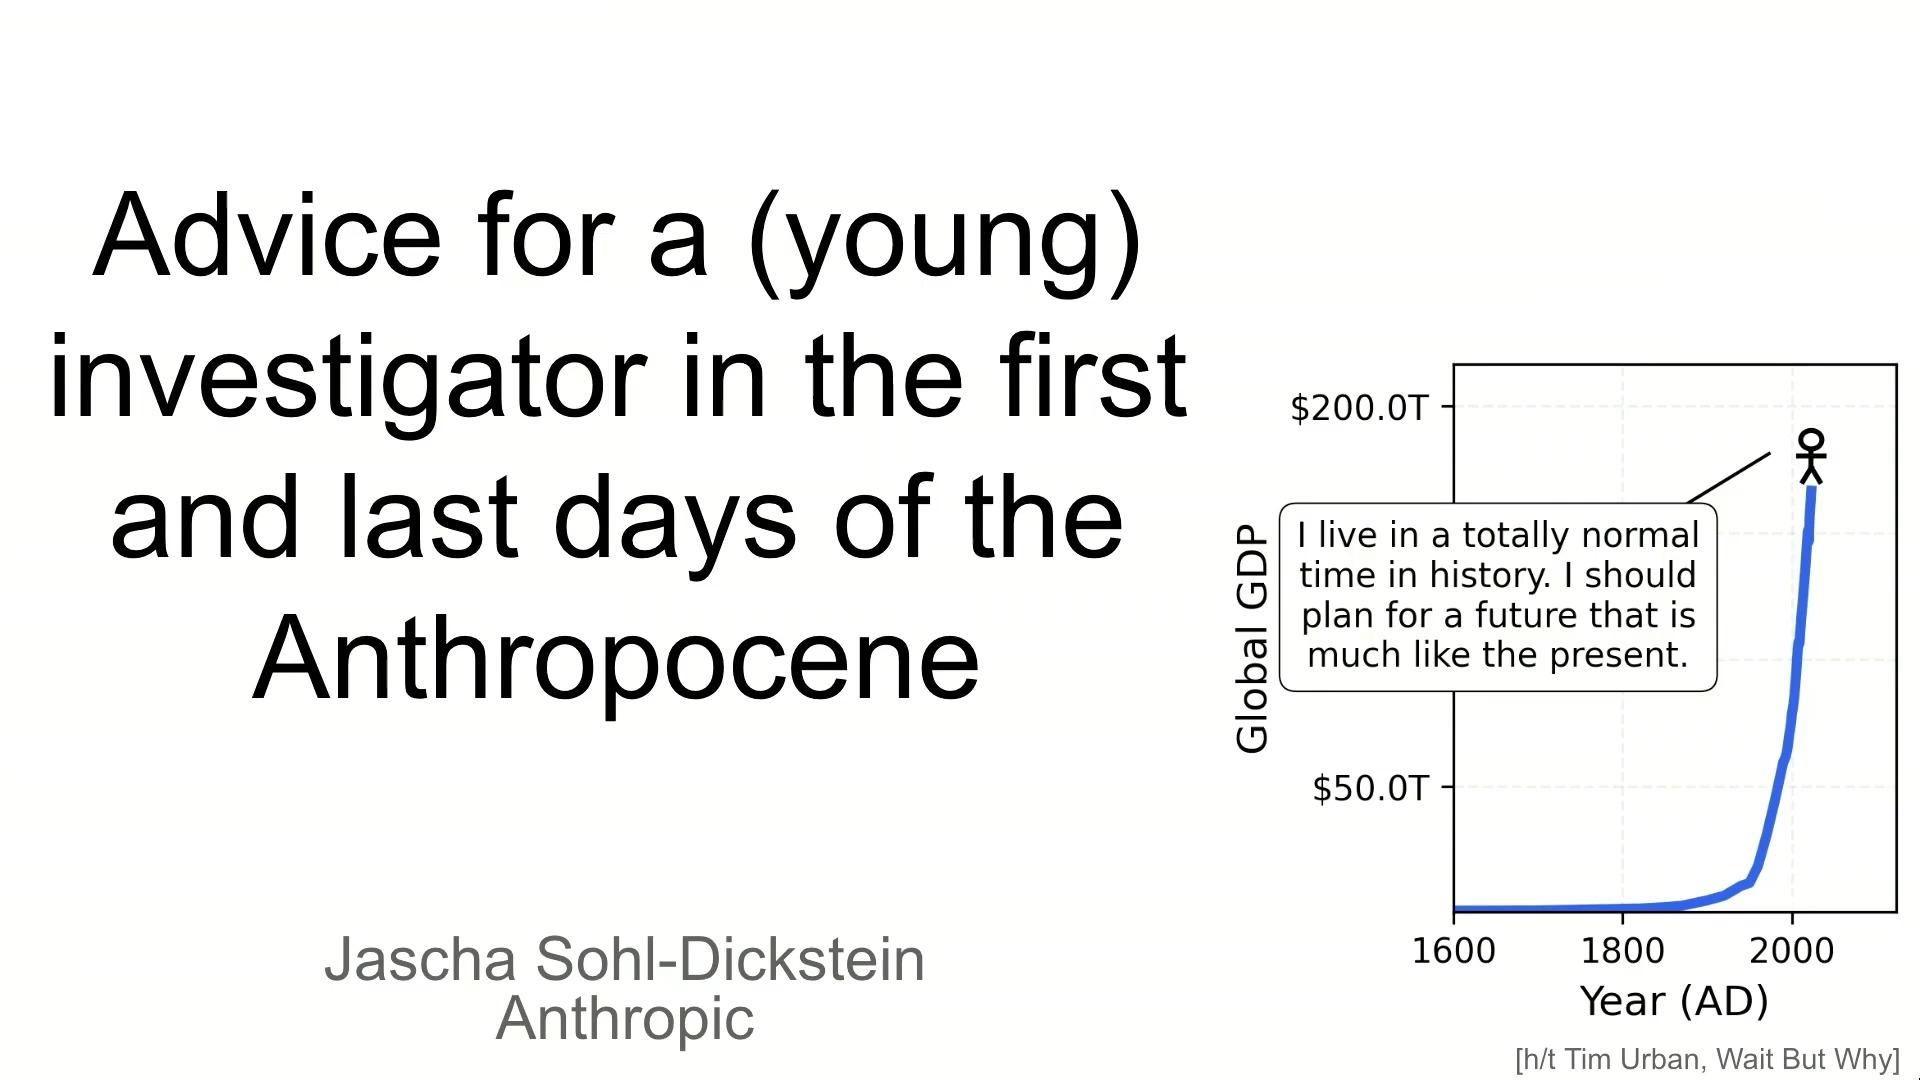
\includegraphics[width=0.92\textwidth]{figures/fig_01_title_gdp_curve.jpg}
\caption{报告开篇标题页：引用 Tim Urban（Wait But Why）绘制的公元 1600--2000 年全球 GDP 曲棍球棒曲线，揭示人类在指数陡峭上升段仍习惯按线性直觉规划未来的认知盲区\vtag}
\end{figure}
\srcnote{00:00:15--00:01:05}

为了直观展现人类直觉在指数增长面前的失灵，Sohl-Dickstein 在开篇引用了科普作家 Tim Urban（\textit{Wait But Why}）著名的历史曲线图（见上图）。图中横轴为公元年份（1600 年至 2000 年），纵轴为全球生产总值（Global GDP，刻度从 $\$50.0\text{T}$ 到 $\$200.0\text{T}$）。在长达数千年的农业与早期工业文明中，全球经济总量几乎贴着横轴缓慢爬行；而在 1950 年之后的短短数十年间，曲线如同一面垂直拔起的悬崖直冲云霄。然而，站在曲线最顶端的小人却望着脚下说道：“我生活在历史上一个再普通不过的时代，我应当按照未来与现在差不多的假设来规划人生。”这种用局部线性切线外推指数悬崖的心理惯性，正是当前学术界在规划科研选题与职业路径时最普遍的认知陷阱。

\begin{figure}[H]
\centering
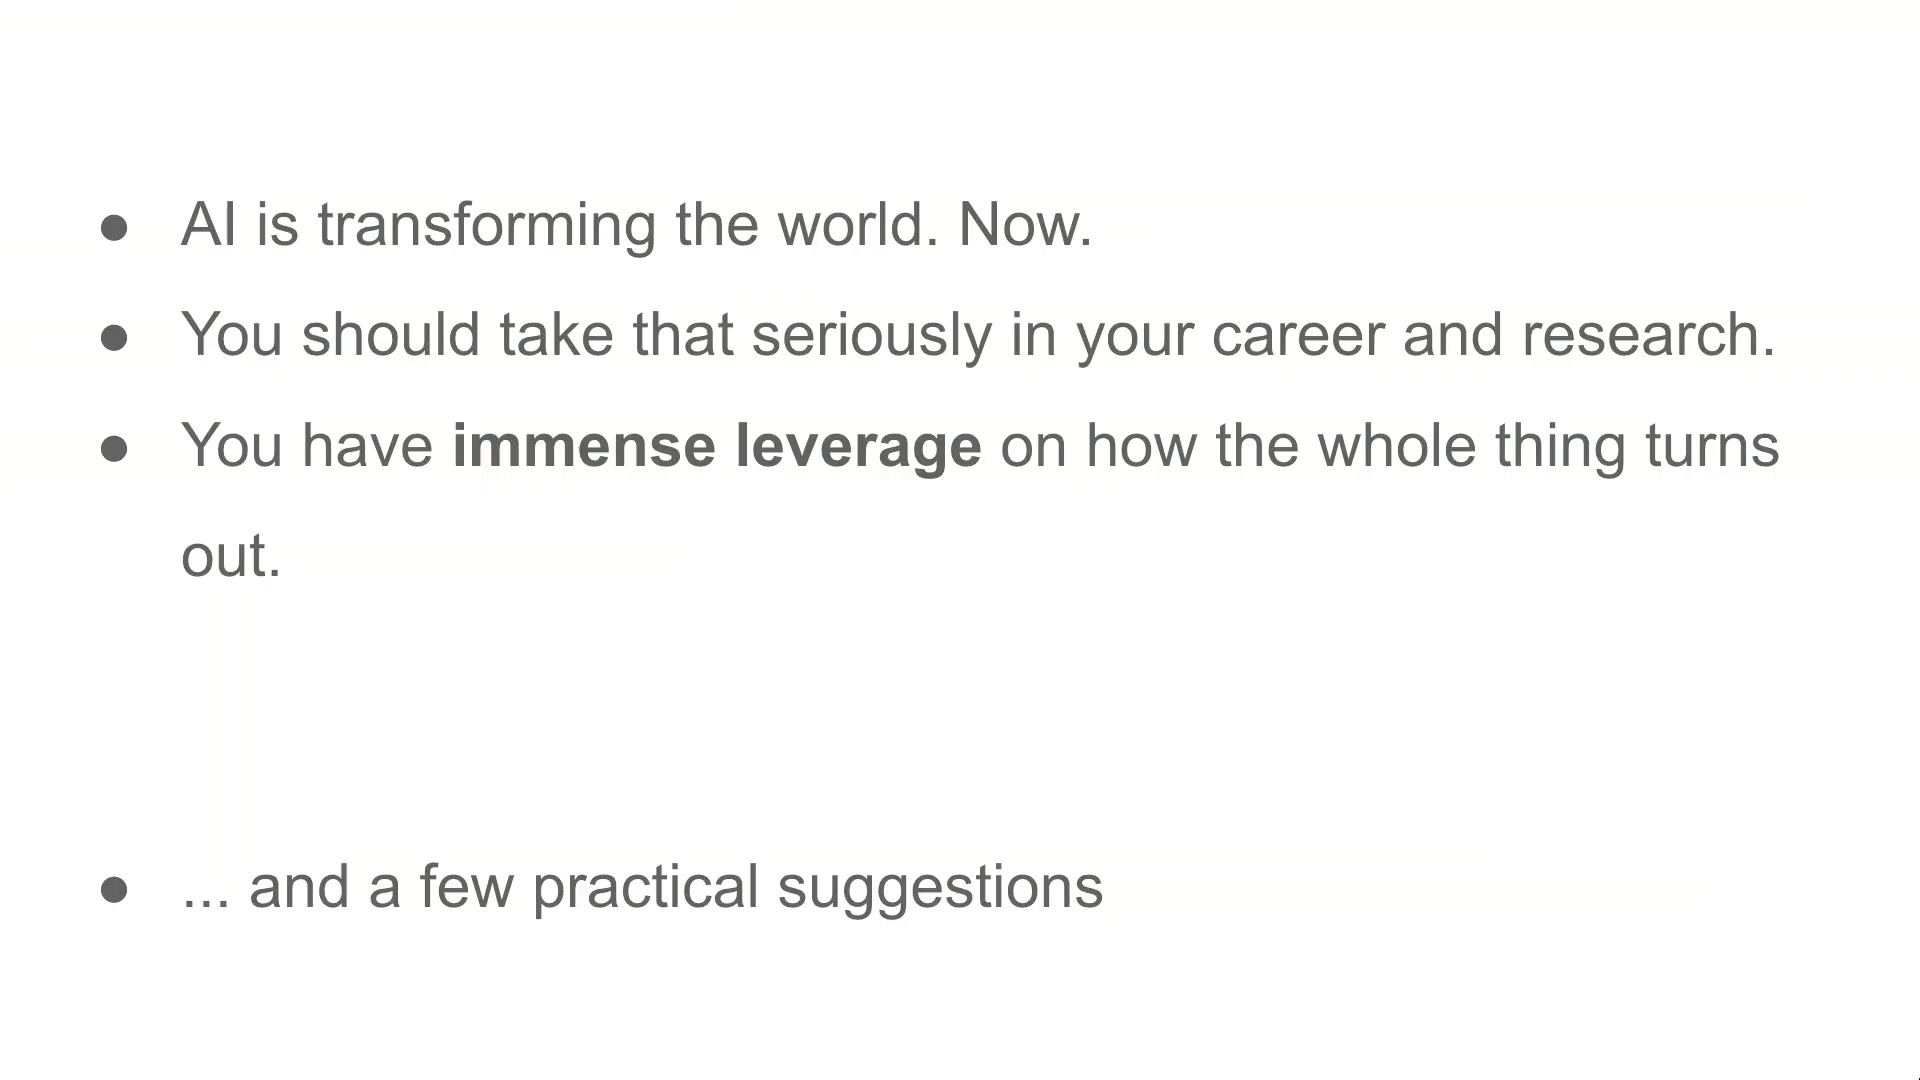
\includegraphics[width=0.92\textwidth]{figures/fig_02_core_thesis.jpg}
\caption{报告的四大核心论点总纲：AI 正在当下重塑世界、研究者必须在职业与科研中严肃对待这一现实、个体对最终走向拥有巨大杠杆，以及若干务实行动建议\vtag}
\end{figure}
\srcnote{00:01:05--00:01:50}

围绕这一历史方位，讲者在第二张幻灯片中明确列出了整场报告的四条核心主线：
\begin{enumerate}
    \item \textbf{AI 正在重塑世界，而且就发生在当下（Now）}：这不是遥远未来的科幻假说，而是已经体现在算力规模、工程任务时长与前沿数学定理证明中的客观事实。
    \item \textbf{你必须在自己的职业生涯与科研规划中严肃对待这一现实}：口头承认技术剧变、行动上却沿用二十年不变的传统学术晋升模板，会导致严重的策略失效。
    \item \textbf{你对整件事最终如何收场拥有巨大的杠杆（Immense Leverage）}：由于我们仍处于指数曲线极其早期的阶段，个体研究者在今日做出的微小选择将被后续的万倍扩张急剧放大。
    \item \textbf{面向未来 1--5 年的具体务实建议}：在选题尺度、工具驾驭、风险权衡与高价值研究方向上给出可落地的操作指南。
\end{enumerate}

\begin{figure}[H]
\centering
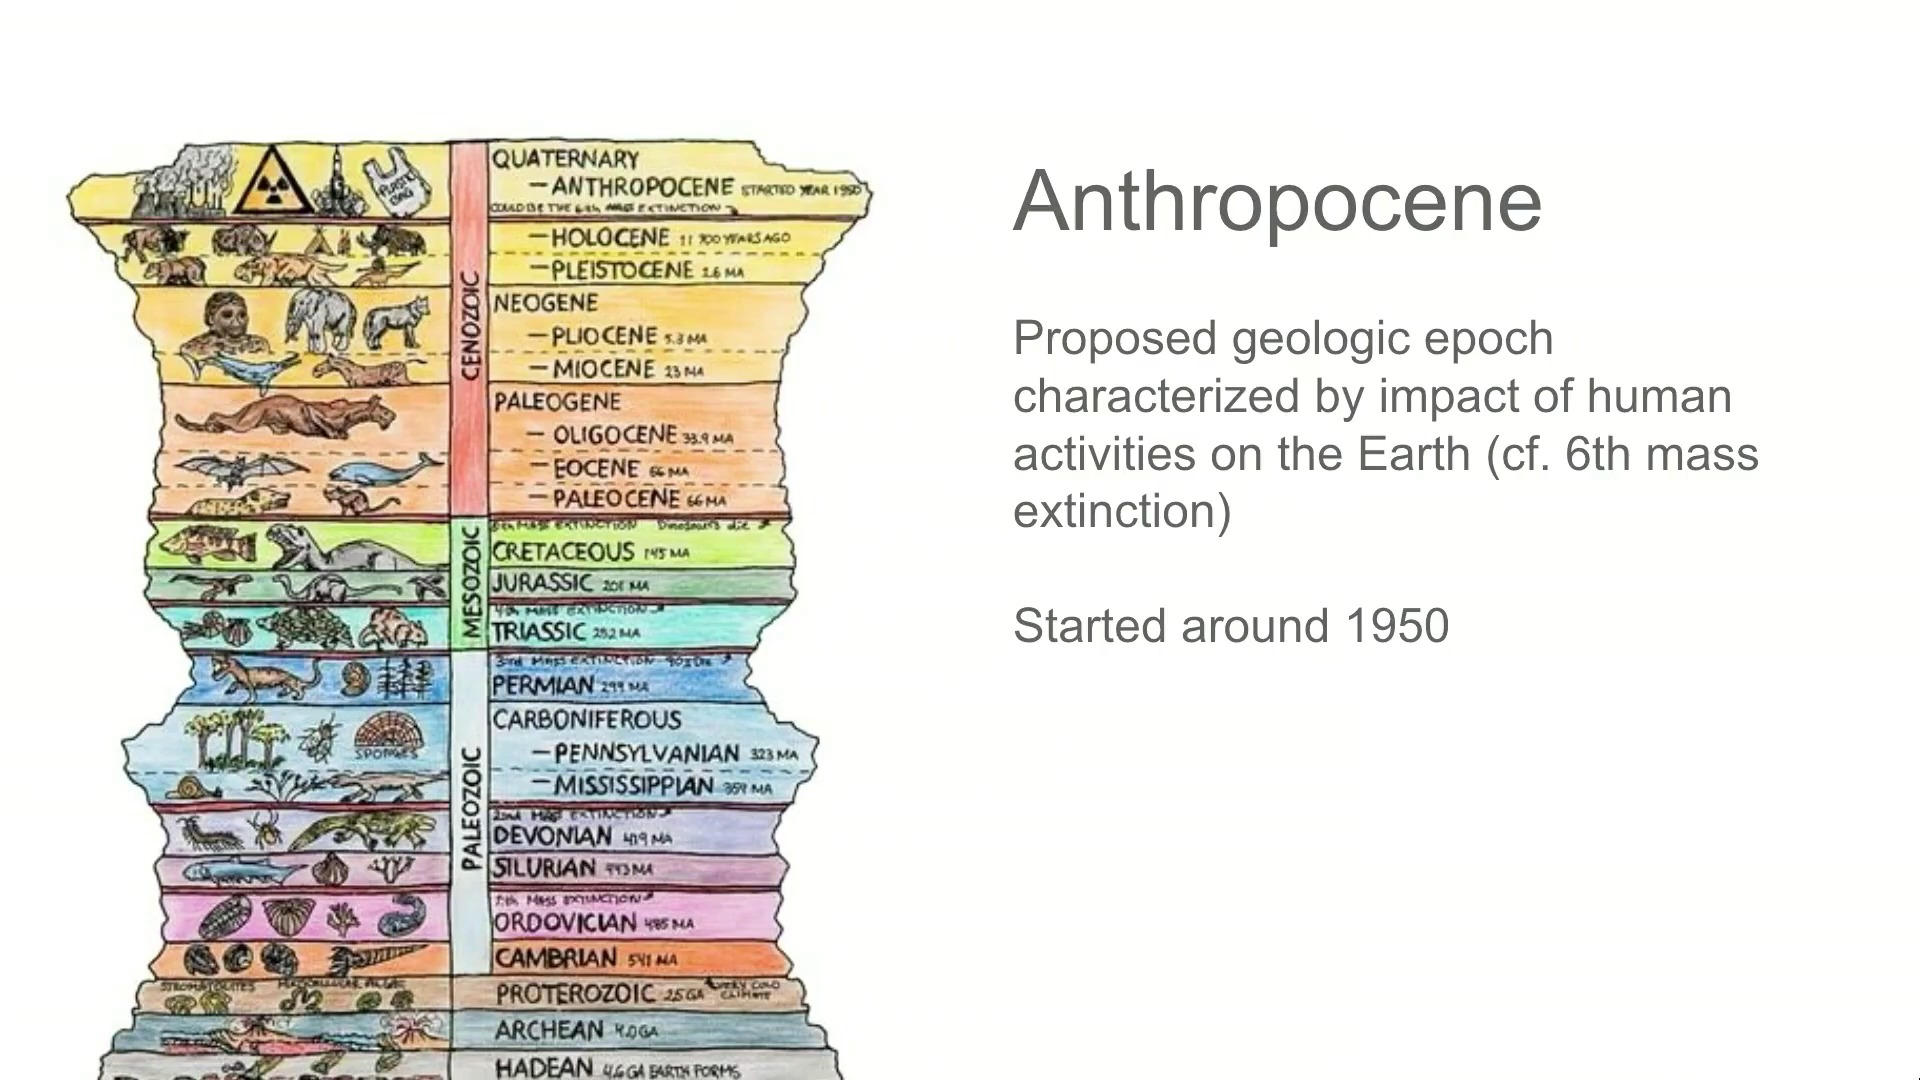
\includegraphics[width=0.92\textwidth]{figures/fig_03_anthropocene_strata.jpg}
\caption{“人类世（Anthropocene）”地质年代柱状图：从冥古宙（Hadean，46 亿年前）到显生宙第四纪，始于 1950 年前后的“人类世”以核爆放射性沉积、塑料污染与第六次物种大灭绝为地层标志\vtag}
\end{figure}
\srcnote{00:02:15--00:03:00}

为什么标题中将当下称为“人类世的最初与最后时日（the first and last days of the Anthropocene）”？讲者借助地质地层柱状图解释道：在地球约 46 亿年（$4.6\text{ GA}$）的演化史中，冥古宙、太古宙、元古宙与显生宙的各个纪元动辄延续数千万乃至数亿年；即便是最近的全新世（Holocene）也始于约 11,700 年前。而地质学家拟议的“人类世（Anthropocene）”则以人类活动对地球表面造成可观测的永久地质印记为界——包括大气碳同位素偏移、微塑料颗粒沉积、人工核试验放射性核素层，以及正在发生的地球第六次生物大灭绝，其起点被定在 \textbf{1950 年}左右。

\begin{knowledgebox}{概念辨析：为什么“人类世”可能成为地球历史上最短的地质纪元？}
按地质学尺度衡量，始于 1950 年的人类世至今尚不足一百年，仅仅是人类数代人的时间跨度，因此今天无疑仍是人类世的“最初时日（first days）”。但与此同时，1950 年也恰好是图灵发表《计算机器与智能》、克劳德·香农制造迷宫机械鼠 Theseus 的人工智能力量起点。讲者指出，一旦通用人工智能（AGI）与超级智能在未来数年至数十年内接管科学与工程的主导权，地球地层与行星能量利用的主导力量将不再是生物意义上的智人（Homo sapiens），而将迈入某种“后人类世（Post-Anthropocene）”。从这个意义上说，我们既身处人类世的黎明，也极可能正站在它落幕的前夜。
\end{knowledgebox}

\subsection{本章小结}
本章通过卡哈尔《致青年研究者》的百年对照与 Tim Urban 的全球 GDP 指数曲线，揭示了人类在指数拐点处“以过去线性外推未来”的普遍盲区，阐明了“人类世（始于约 1950 年）”在地质尺度与技术尺度上的双重涵义，并确立了报告围绕“实证趋势—时间线共识—个人行动策略—历史级杠杆”展开的四层论证框架。

\clearpage
\section{人类世的 AI 指数跃迁：算力、任务跨度与数学发现}

为了说明“AI 正在重塑世界”并非主观臆测，Sohl-Dickstein 从底层投入（训练算力）、工程产出（软件任务自主完成时长）与基础科学突破（开放 Erdős 数学猜想求解）三个相互独立的定量维度展示了跨数量级的指数曲线。

\subsection{训练算力的两阶段指数增长与人脑毕生算力基准}

第一项核心证据来自 Our World in Data 统计的 1950--2025 年人工智能模型训练算力（Training computation，单位为 $\text{petaFLOP}$，即 $10^{15}$ 次浮点运算）对数坐标图。由于纵轴采用对数刻度，图中的直线直接对应指数增长（Exponential Growth）。

\begin{figure}[H]
\centering
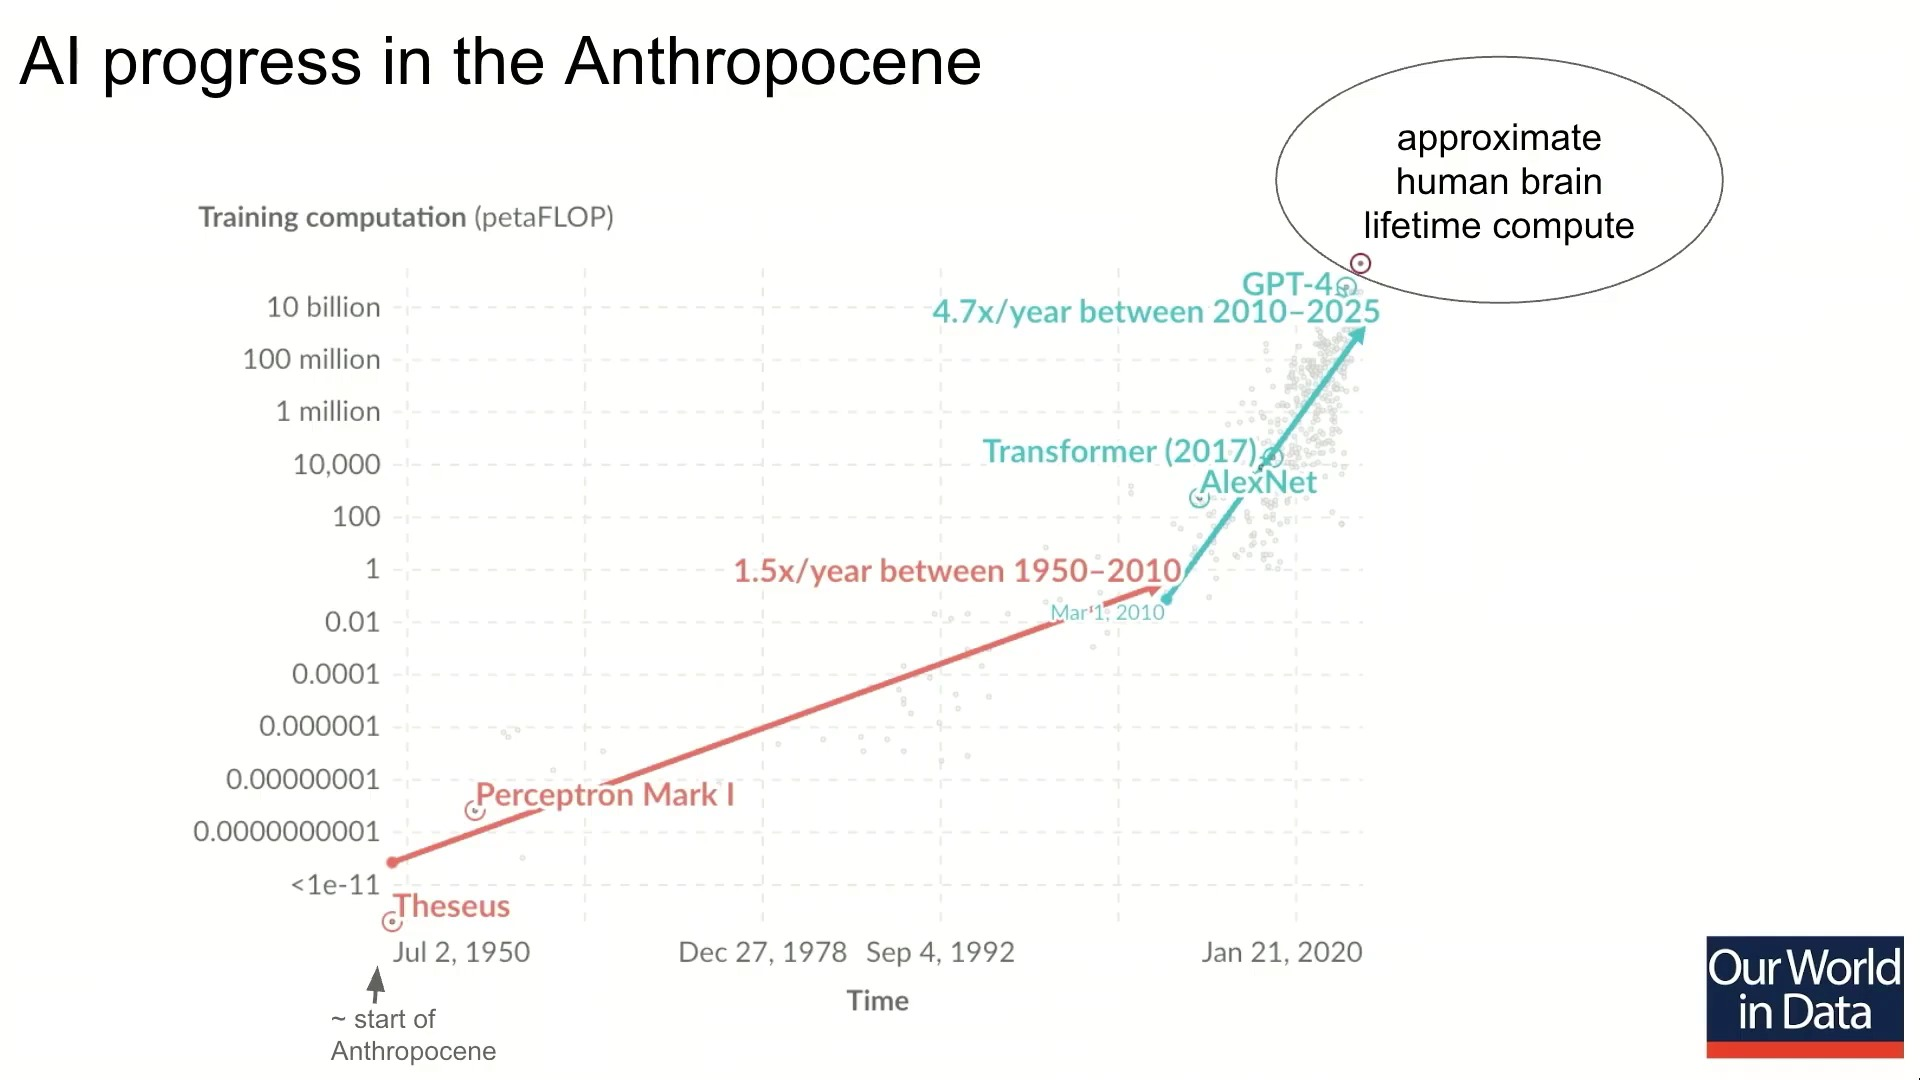
\includegraphics[width=0.92\textwidth]{figures/fig_04_training_compute.jpg}
\caption{人类世的 AI 训练算力演进（1950--2025）：从 1950--2010 年的年均 $1.5\times$ 增长跃升至 2010--2025 年的年均 $4.7\times$ 增长，右上角椭圆标出了人脑毕生总算力的粗略估算区间\vtag}
\end{figure}
\srcnote{00:03:30--00:05:30}

从图中可以清晰辨识出两个斜率截然不同的历史阶段：
\begin{itemize}
    \item \textbf{第一阶段（1950--2010 年，摩尔定律驱动期）}：从 1950 年 7 月 2 日香农的 Theseus（算力低于 $10^{-11}\text{ petaFLOP}$，恰与人类世起点重合）与 1950 年代末的感知机 Perceptron Mark I 开始，直至 2010 年 3 月深度学习爆发前夕，前沿 AI 模型的训练算力以每年约 \textbf{$1.5\times$（1.5 倍/年）} 的速率稳步指数攀升。
    \item \textbf{第二阶段（2010--2025 年，深度学习与大模型规模化期）}：自 2010 年起，经由 AlexNet（2012）、Transformer（2017）直至 GPT-4 等前沿基础模型，训练算力的增长斜率急剧变陡，达到惊人的每年 \textbf{$4.7\times$（4.7 倍/年）}。在短短 15 年间，单次前沿训练运行所消耗的算力累计增长了约 \textbf{1000 万倍（$10^7\times$，即 10 million fold）}。
\end{itemize}

为了给 $10^{10}\text{ petaFLOP}$（100 亿 petaFLOP）量级的冷冰冰数字提供直觉锚点，讲者在图的右上角用黑色椭圆圈出了一个关键物理参照系——\textbf{单个人类大脑在一生中所执行的总计算量（Approximate human brain lifetime compute）}。在报告现场，他给出了这一量级的信封背面估算（Back-of-the-envelope estimate）：

\[
\begin{aligned}
C_{\text{brain, lifetime}} &\approx N_{\text{syn}} \cdot f_{\text{op}} \cdot T_{\text{life}} \approx 10^{15} \times 1\text{ FLOP/s} \times \left(80 \times 3.15 \times 10^7\text{ s}\right) \\
&\sim 10^{25}\text{--}10^{27}\text{ FLOP} \approx 10^{10}\text{--}10^{12}\text{ petaFLOP}
\end{aligned}
\]

式中各符号的物理意义与量级取法如下：
\begin{itemize}
    \item $C_{\text{brain, lifetime}}$：单个人脑在整个生命周期内完成的等效浮点运算总数（以 FLOP 或 petaFLOP 计量，其中 $1\text{ petaFLOP} = 10^{15}\text{ FLOP}$）；
    \item $N_{\text{syn}} \approx 10^{15}$：人脑皮层与皮层下结构中包含的突触（Synapses）总数量级；
    \item $f_{\text{op}} \sim 1\text{--}10^2\text{ FLOP/s}$：单个突触每秒钟有效脉冲传递与突触权重更新所折算的等效浮点操作频率（受神经元平均发放率约 $1\text{--}10\text{ Hz}$ 约束）；
    \item $T_{\text{life}} \approx 2.5 \times 10^9\text{ s}$：人类约 80 年寿命对应的秒数（即便把童年发育、睡眠与日常非学术思考全部计入）。
\end{itemize}

这一估算揭示了一个令人震撼的事实：即便算法效率完全不做优化，当前最前沿大模型的单次预训练算力（已跨入 $10^{10}\text{--}10^{11}\text{ petaFLOP}$ 区间）就已经与一个人从出生到老死大脑运转的全部突触计算总量处于同一数量级。

\subsection{METR 软件工程任务时间跨度的指数延长}

算力只是投入侧的度量；在产出侧，AI 究竟能独立完成多复杂的真实工作？讲者随后展示了评估机构 METR（Model Evaluation and Threat Research）的里程碑研究图表（见下图）。

\begin{figure}[H]
\centering
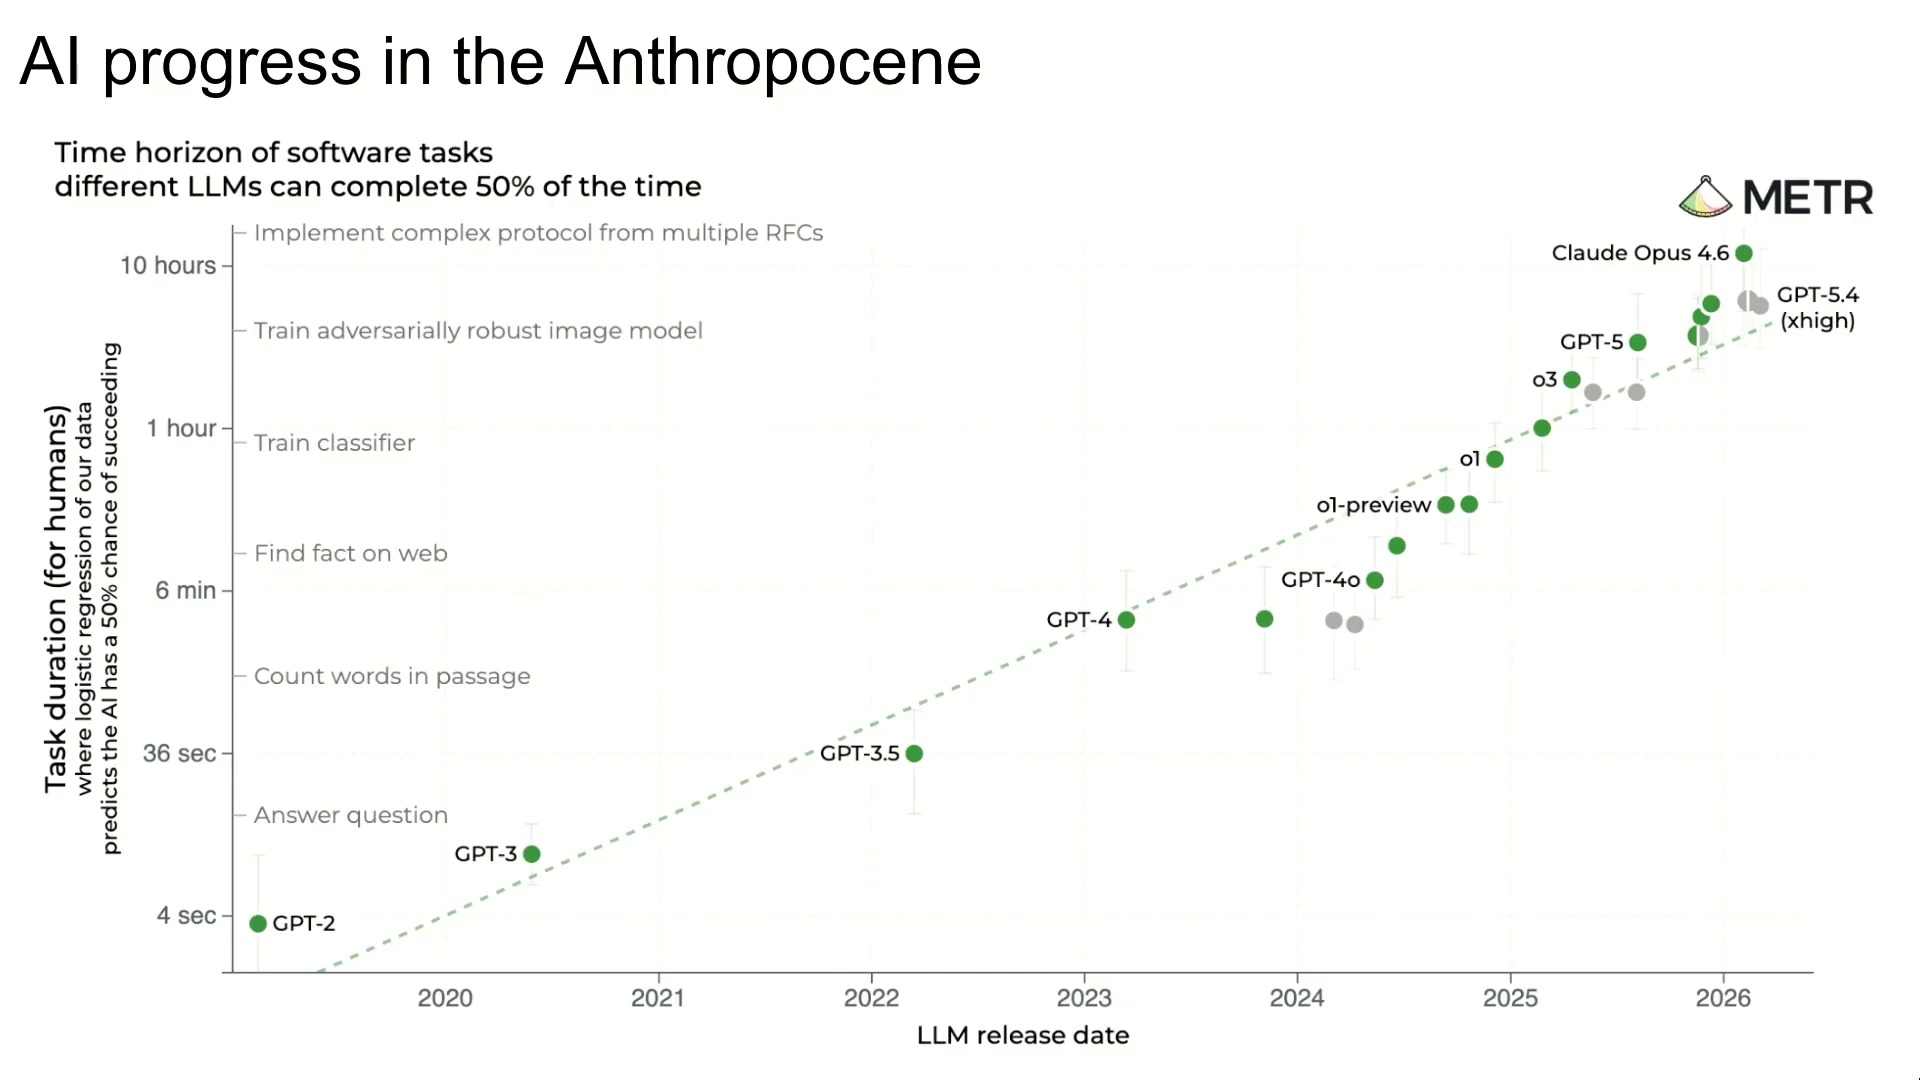
\includegraphics[width=0.92\textwidth]{figures/fig_05_metr_task_horizon.jpg}
\caption{METR 软件工程任务时间跨度演进图：纵轴为人类工程师完成该任务所需的时长，数据点表示不同发布年份的 LLM 能够以 50\% 成功率独立完成的任务时间跨度\vtag}
\end{figure}
\srcnote{00:05:30--00:06:55}

在这张图中，横轴为大语言模型的发布日期（2020 年至 2026 年），纵轴采用对数刻度，表示\textbf{一名熟练人类软件工程师完成某项软件工程任务所需的时间}（从 4 秒、36 秒、6 分钟、1 小时直到 10 小时以上），而图中每个模型的位置则对应逻辑回归预测该模型能够以 \textbf{50\% 成功率（50\% of the time）}独立做完的任务难度：
\begin{itemize}
    \item \textbf{2019--2020 年（GPT-2 / GPT-3）}：GPT-2 仅能完成人类耗时约 \textbf{4 秒}的微任务（如直接回答一个简单问题）；GPT-3 提升至十余秒量级。
    \item \textbf{2022--2023 年（GPT-3.5 / GPT-4）}：GPT-3.5 跨过 \textbf{36 秒}门槛（如清点一段文本的词数）；GPT-4 与随后的 GPT-4o 达到约 \textbf{6 分钟}人类工时水平（如在网页上检索并核实特定事实）。
    \item \textbf{2024--2025 年初（o1-preview / o1）}：推理模型的引入使有效任务跨度逼近 \textbf{1 小时}（如独立编写代码并训练一个分类器）。
    \item \textbf{2025--2026 年初（o3 / GPT-5 / GPT-5.4 xhigh / Claude Opus 4.6）}：任务时间跨度沿着对数直线一路向上突破数小时乃至 \textbf{10 小时}大关（如训练具备对抗鲁棒性的图像分类模型、阅读多份互联网工程任务组 RFC 文档并完整实现一套复杂通信协议）。
\end{itemize}

讲者特别补充指出，虽然图上主线采用的是 50\% 成功率阈值，但研究人员同时测算了模型能够以 \textbf{80\%} 把握（80\% likely to do）甚至 \textbf{90\%} 高可靠性（fully or like 90\% reliability）完成的任务时长曲线——除了整体在纵轴上向下平移一个常数截距外，80\% 与 90\% 可靠性曲线的指数增长斜率与 50\% 曲线完全一致（约每 7 个月翻一番）。将这条对数直线向后外推短短数年，AI 能够独立闭环执行的软件与科研工程跨度就将从“一天”扩展到“数周、数月乃至一整年的博士课题”。

\subsection{开放 Erdős 数学猜想的 AI 求解爆发：七个月从 0 到 56}

如果说软件工程任务还包含大量常规编码工作，那么纯数学领域的开放猜想则是人类抽象创造力的试金石。二十世纪传奇数学家保罗·爱多士（Paul Erdős）生前提出了上千个跨越组合数学、数论与图论的开放问题（Erdős Problems），其中许多问题悬赏数十年未果。

\begin{figure}[H]
\centering
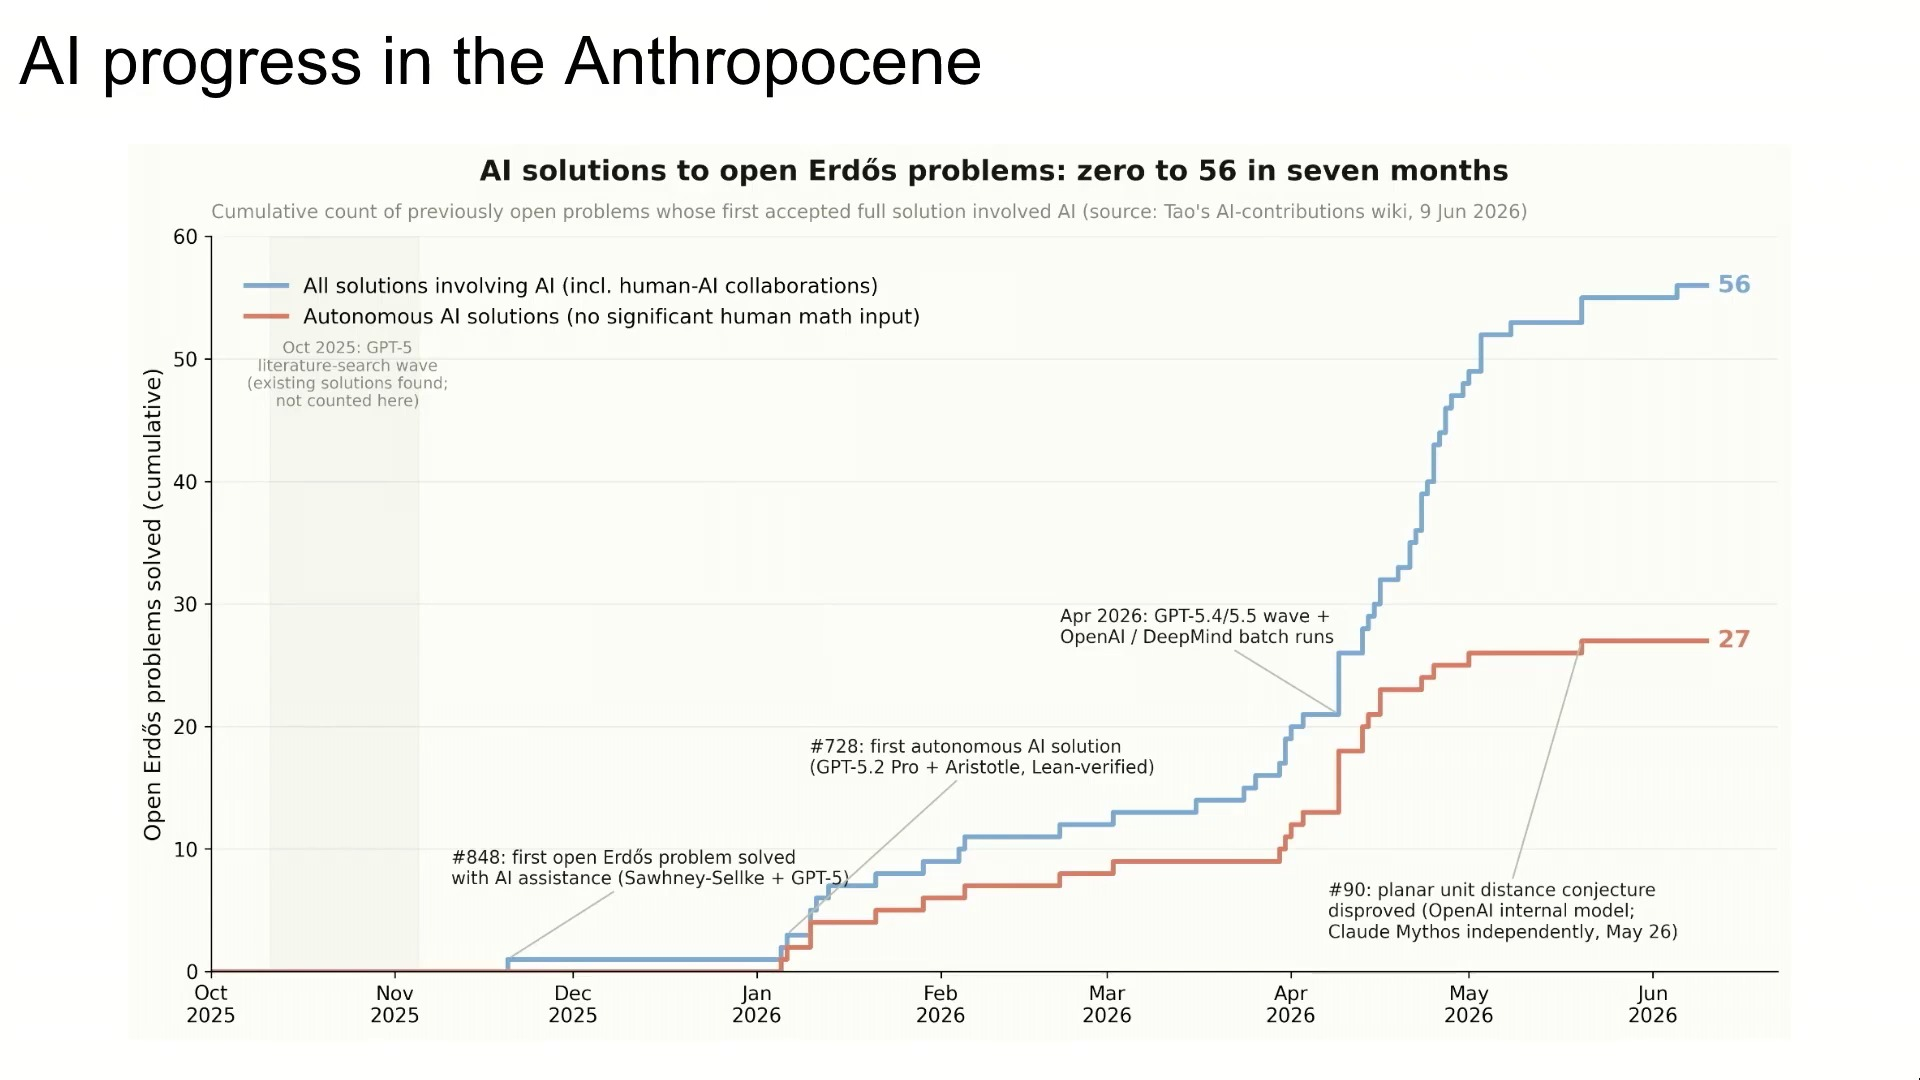
\includegraphics[width=0.92\textwidth]{figures/fig_06_erdos_problems.jpg}
\caption{开放 Erdős 数学问题的 AI 求解累计曲线（数据源：陶哲轩 AI-contributions wiki，截至 2026 年 6 月 9 日）：7 个月内共有 56 个此前未解的 Erdős 问题在 AI 参与下首次获解，其中 27 个为无显著人类数学输入的 AI 全自主求解\vtag}
\end{figure}
\srcnote{00:06:55--00:08:20}

上图汇总了菲尔兹奖得主陶哲轩（Terence Tao）维护的 AI 数学贡献维基（截至 2026 年 6 月 9 日）的统计记录。在 2025 年 11 月之前，由 AI 实质性参与并首次给出完整解答的开放 Erdős 问题数量严格为 \textbf{0}（注：2025 年 10 月曾出现一波利用 GPT-5 进行深度文献检索、找回历史上已被人类证明但未被题库收录之解答的浪潮，图中灰色阴影区已将其严格剔除，不计入新解）。然而，从 2025 年 11 月底到 2026 年 6 月初的短短\textbf{七个月}内，累计曲线呈现爆发式阶跃：
\begin{enumerate}
    \item \textbf{2025 年 11 月底（问题 \#848）}：数学家 Sawhney 与 Sellke 借助 GPT-5 完成了首个由 AI 辅助攻克的开放 Erdős 问题。
    \item \textbf{2026 年 1 月（问题 \#728）}：GPT-5.2 Pro 结合形式化证明系统 Aristotle，给出了首个\textbf{无显著人类数学输入（No significant human math input）}并通过 Lean 形式化验证的全自主 AI 证明。
    \item \textbf{2026 年 4 月（批量求解潮）}：随着 GPT-5.4/5.5 的发布以及 OpenAI 与 DeepMind 开展系统性批量运行（Batch runs），获解问题数在数周内陡增数十项。
    \item \textbf{2026 年 5 月 26 日（问题 \#90）}：著名的平面单位距离猜想（Planar unit distance conjecture）被 OpenAI 内部模型与 Anthropic 的 Claude Mythos 模型各自独立证伪。
\end{enumerate}

截至统计日，包含人机协作在内的 AI 获解 Erdős 开放问题总数已达 \textbf{56} 项（蓝线），其中完全不依赖人类数学家构思的 AI 自主求解达 \textbf{27} 项（红线）。Sohl-Dickstein 结合自身体会坦言：一年前他还亲手编写绝大部分实验代码；半年前他退居为“从不自己写代码、只给 Claude 布置任务的微管理导师”；而到了最近几周，他发现直接向 Claude 提出高层次科学问题、让模型自行设计实验、运行分析并生成可视化图表，其产出效率已经远超自己亲自下场。

\begin{table}[H]
\centering
\small
\caption{人类世 AI 指数跃迁的三大核心实证维度汇总}
\begin{tabular}{p{2.6cm}p{3.2cm}p{3.6cm}p{4.2cm}}
\toprule
\textbf{评估维度} & \textbf{历史基线} & \textbf{当前前沿水平（2025--2026）} & \textbf{指数增长率与核心里程碑} \\
\midrule
前沿训练算力\newline（Our World in Data） & 1950 年 Theseus $<10^{-11}\text{ petaFLOP}$；1950--2010 年均增长 $1.5\times$ & 单次训练达 $10^{10}\text{--}10^{11}\text{ petaFLOP}$ 量级 & 2010--2025 年均增长 \textbf{$4.7\times$}（15 年增 1000 万倍），逼近人脑毕生算力（$\sim 10^{12}\text{ petaFLOP}$） \\
软件任务时间跨度\newline（METR 50\% 阈值） & 2019 年 GPT-2 仅能完成约 \textbf{4 秒}人类微任务 & Claude Opus 4.6 / GPT-5.4 可完成约 \textbf{10 小时}复杂工程任务 & 50\%、80\% 与 90\% 可靠性曲线均呈对数线性增长，任务跨度约每 7 个月翻倍 \\
开放 Erdős 猜想\newline（Tao Wiki 统计） & 2025 年 11 月前 AI 实质求解数为 \textbf{0} & 7 个月内累计攻克 \textbf{56} 题，其中 AI 全自主求解 \textbf{27} 题 & 含 \#848（首个人机协作解）、\#728（首个 Lean 验证自主解）与 \#90（平面单位距离猜想证伪） \\
\bottomrule
\end{tabular}
\end{table}

\subsection{本章小结}
本章从算力投入、软件工程自主时长与前沿数学定理证明三个维度立起了不可辩驳的数据支柱：训练算力在过去 15 年以年均 $4.7\times$ 的速度激增 1000 万倍并逼近人脑毕生算力（$\sim 10^{12}\text{ petaFLOP}$）；LLM 可靠完成的软件工程任务时长从秒级跨越至 10 小时级；开放 Erdős 数学难题在 7 个月内被攻克 56 项（27 项全自主）。三条独立对数直线的同步陡升，构成了判断未来 1--5 年技术走向的客观底座。

\clearpage
\section{奥弗顿之窗的迁移与旧金山实验室的 AGI 时间线}

当底层技术沿着指数曲线疾驰时，社会认知与主流舆论往往存在明显的滞后，但一旦跨过临界点，公共讨论的“奥弗顿之窗（Overton Window，即被主流社会视为合理、可公开讨论的观点范围）”就会发生剧烈位移。

\subsection{从“疯子摘要”邮件到政商领袖与主流媒体的共识}

Sohl-Dickstein 分享了一件极具戏剧性的亲身经历。2025 年 8 月，他在哈佛大学举办了一场题为《人类世初末的青年研究者指南》的特别学术研讨会（Aug 12 Special AM Seminar）。就在讲座海报发出的几天前（2025 年 8 月 4 日），一位素不相识的学者将讲座通知转发给他，并在邮件正文中毫不客气地写道（见下图绿色圆圈标注）：\textbf{“What a bat-shit crazy abstract...（多么疯癫荒谬的讲座摘要……）”}

\begin{figure}[H]
\centering
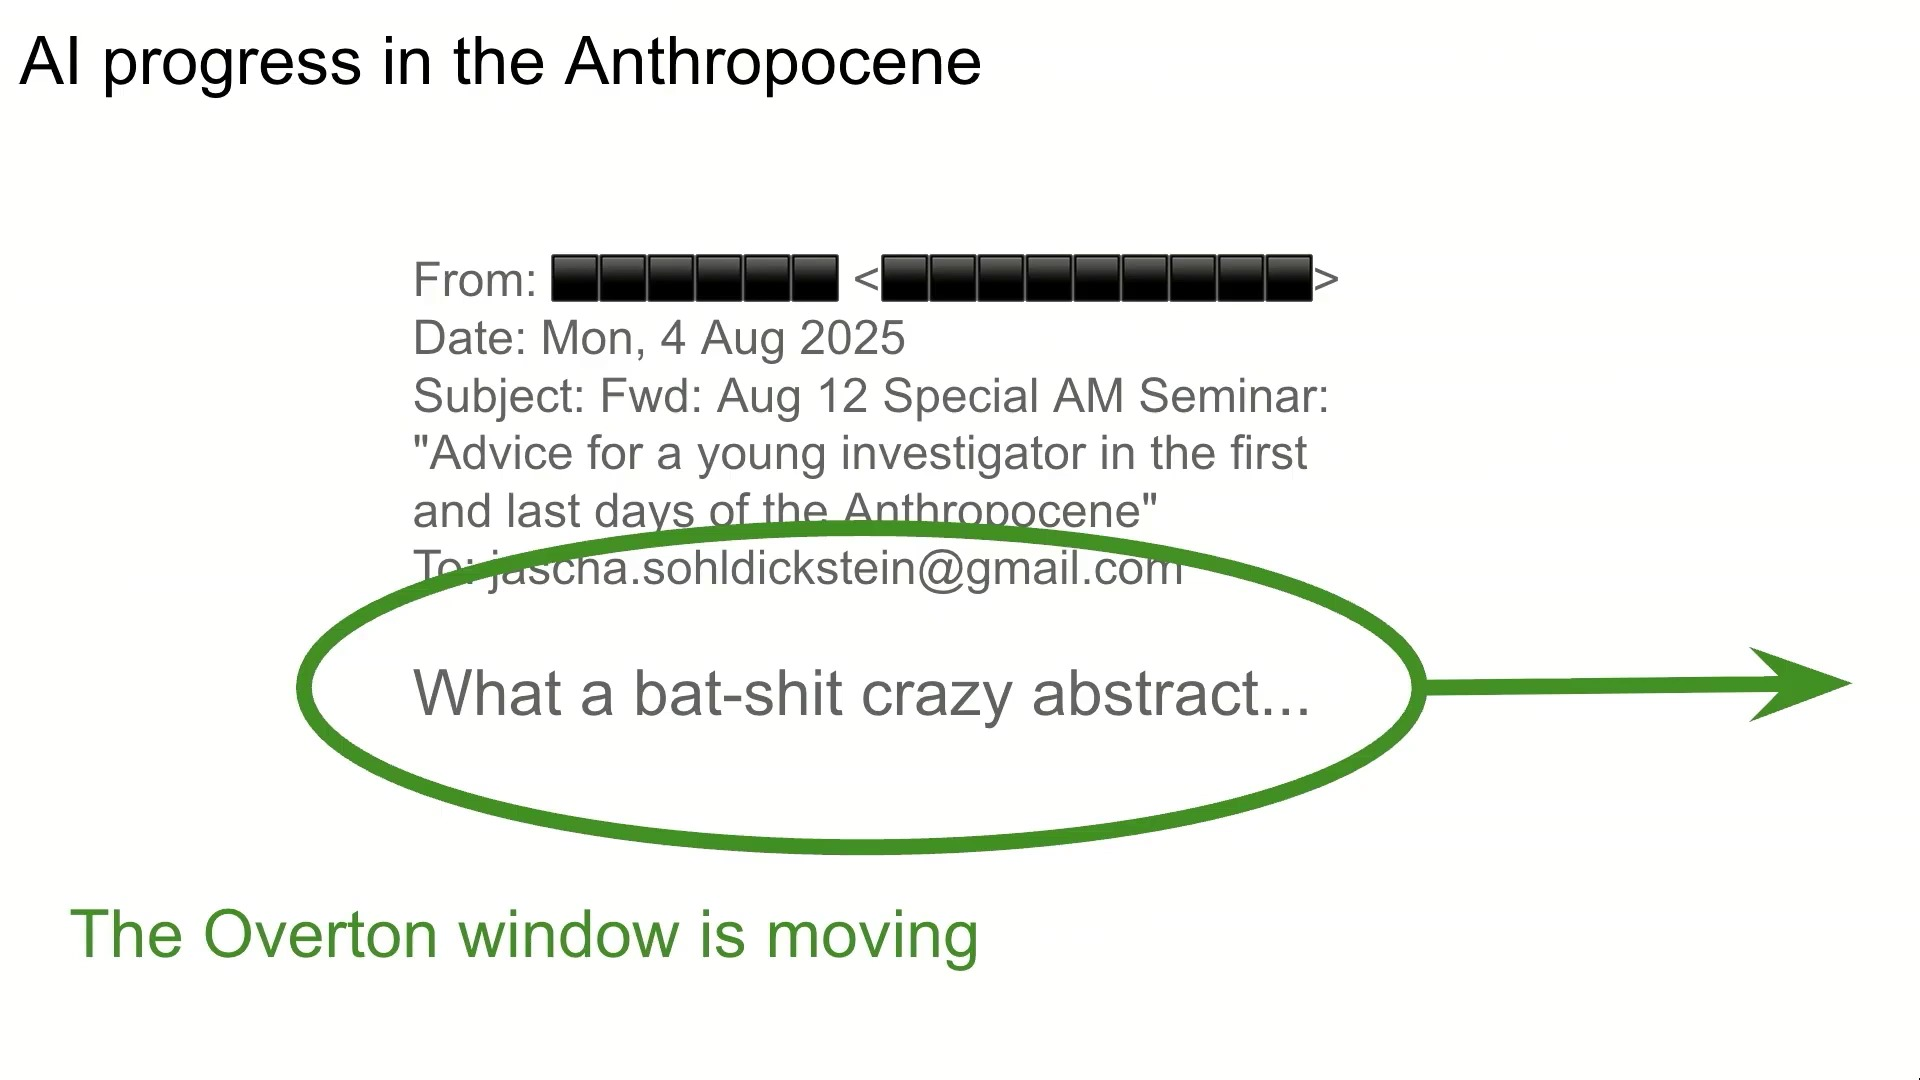
\includegraphics[width=0.90\textwidth]{figures/fig_07_overton_window.jpg}
\caption{2025 年 8 月哈佛研讨会前夕讲者收到的质疑邮件：“What a bat-shit crazy abstract...”，折射出部分传统学者对短期 AGI 时间线的本能排斥与正在移动的奥弗顿之窗\vtag}
\end{figure}
\srcnote{00:09:20--00:10:05}

为什么一位受过良好训练的传统学者会把“严肃规划未来 1--5 年的 AGI 冲击”视为疯言疯语？因为在此前数十年的学术规范中，谈论通用人工智能或超级智能往往被贴上“科幻炒作”的标签。然而，讲者通过随后两张幻灯片展示出，就在短短一年之内，奥弗顿之窗已经从边缘极客圈迅速席卷至全球最高政治与商业决策层。

\begin{figure}[H]
\centering
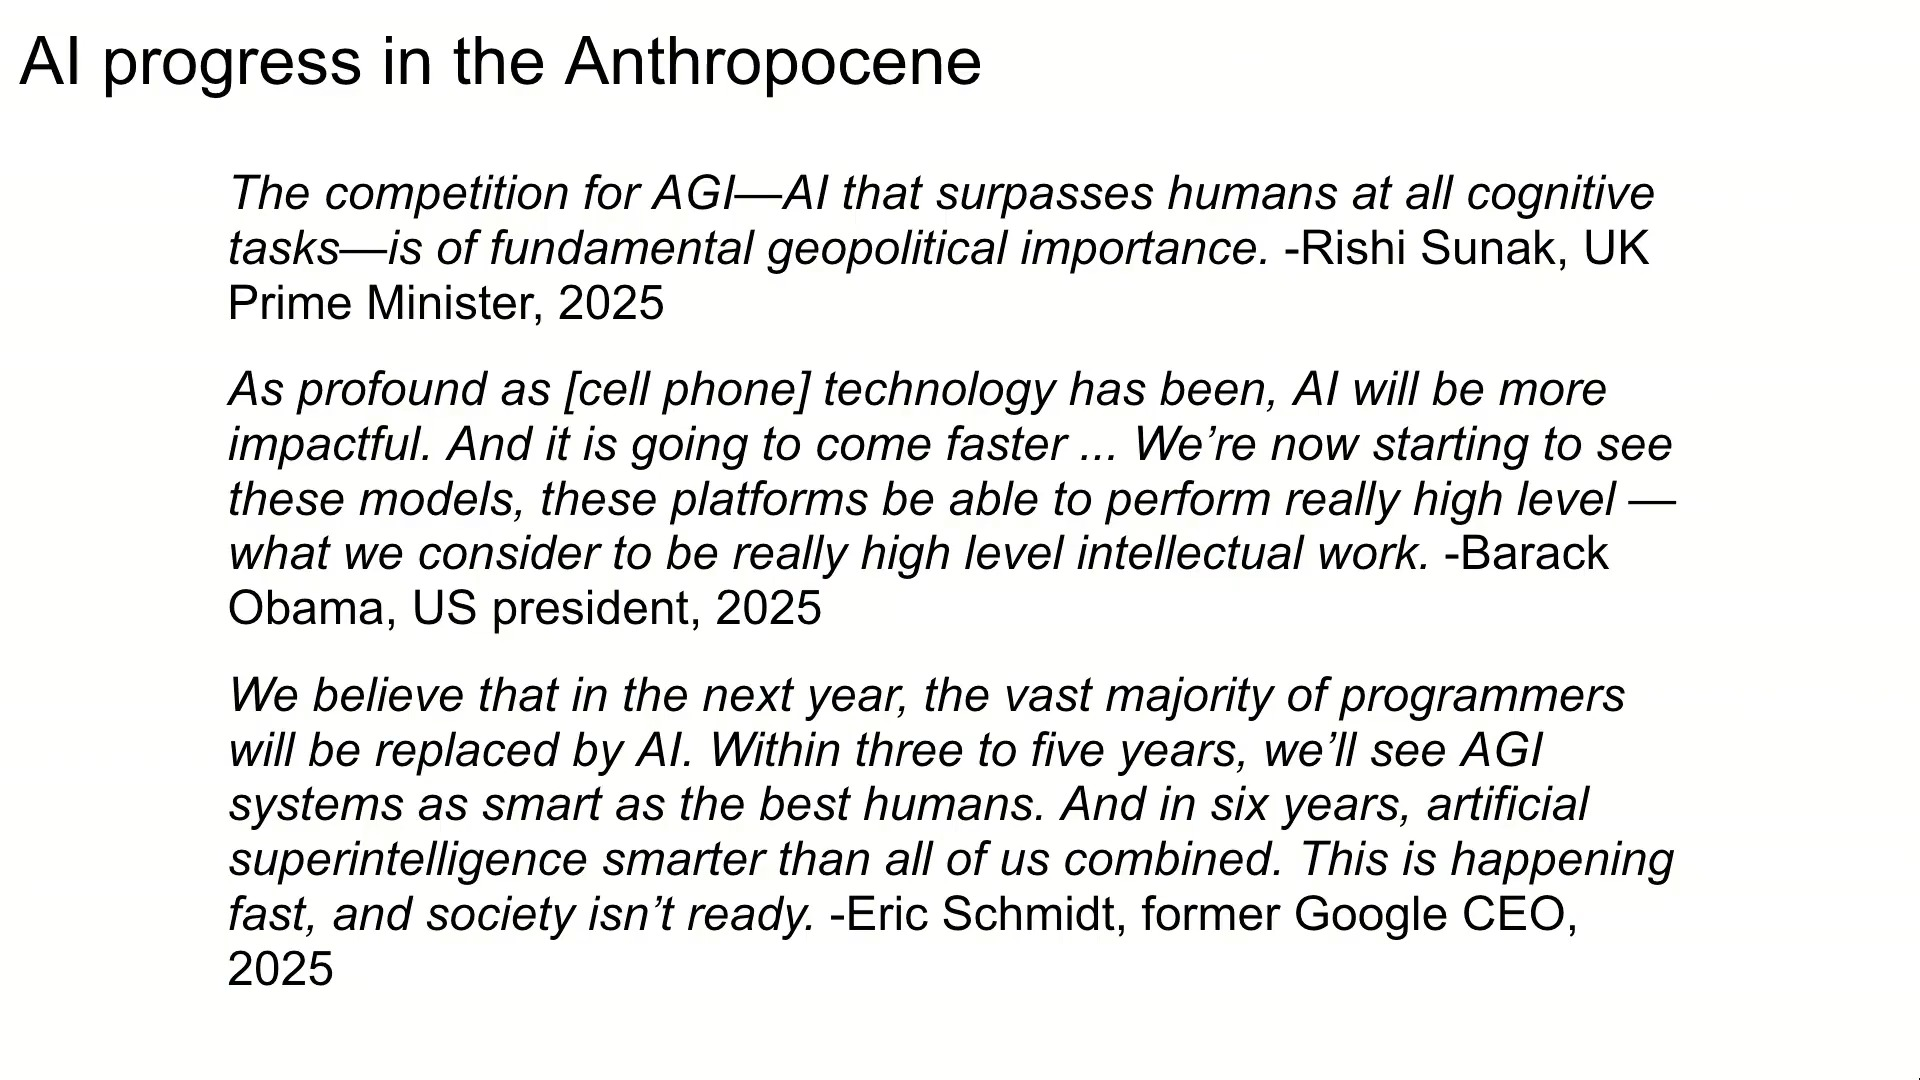
\includegraphics[width=0.92\textwidth]{figures/fig_08_agi_leader_quotes.jpg}
\caption{2025 年全球政商领袖关于 AGI 的公开表态：英国前首相 Rishi Sunak、美国前总统 Barack Obama 与 Google 前首席执行官 Eric Schmidt 的判断\vtag}
\end{figure}
\srcnote{00:10:05--00:11:30}

如上图所示，2025 年的三段标志性公开言论清晰记录了这一认知水位线的抬升：
\begin{itemize}
    \item \textbf{Rishi Sunak（英国首相，2025）}：“围绕 AGI——即在所有认知任务上超越人类的 AI——的竞争，具有根本性的地缘政治重要性。”
    \item \textbf{Barack Obama（美国前总统，2025）}：“尽管智能手机技术的影响已经如此深远，但 AI 的冲击将更为巨大，而且来得更快……我们现在已经开始看到这些模型、这些平台能够执行真正高水平的——被我们视为真正高水平的智力工作（really high level intellectual work）。”
    \item \textbf{Eric Schmidt（Google 前首席执行官，2025）}：“我们相信在未来一年内，绝大多数程序员将被 AI 取代。在三到五年内，我们将看到与最优秀人类一样聪明的 AGI 系统。而在六年内，将出现比我们所有人加起来还要聪明的超级人工智能（ASI）。这一切发生得极快，而整个社会还没有做好准备。”
\end{itemize}

\begin{figure}[H]
\centering
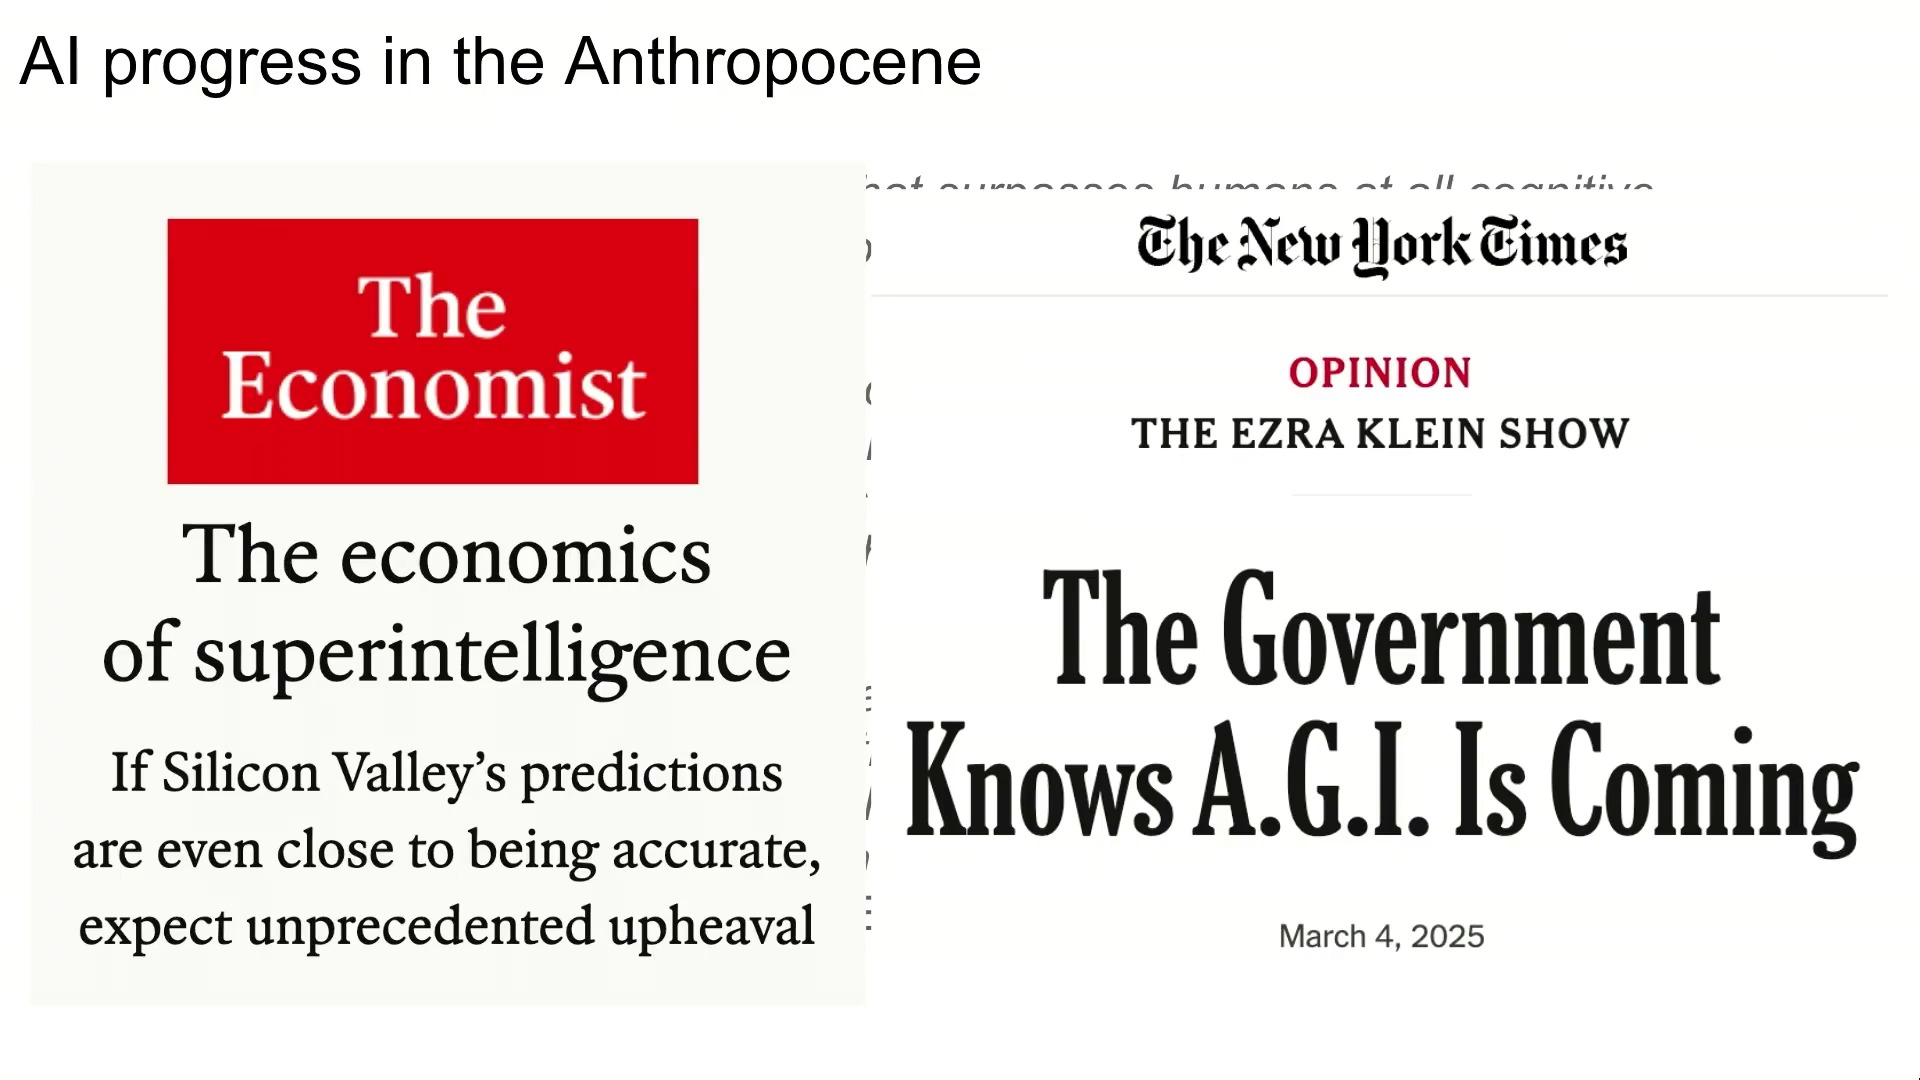
\includegraphics[width=0.92\textwidth]{figures/fig_09_media_shift.jpg}
\caption{主流媒体的议程转向：《经济学人》专题探讨“超级智能经济学”，《纽约时报》Ezra Klein 专栏于 2025 年 3 月 4 日刊文《政府知道 AGI 即将到来》\vtag}
\end{figure}
\srcnote{00:11:30--00:12:05}

与此同时，一向以审慎保守著称的严肃媒体也彻底改变了语调（见上图）：《经济学人》（\textit{The Economist}）刊发重磅专题《超级智能的经济学：如果硅谷的预测哪怕只有几分接近准确，也请准备好迎接前所未有的剧变》；《纽约时报》（\textit{The New York Times}）著名专栏作家 Ezra Klein 则在 2025 年 3 月 4 日直接以《政府知道 AGI 即将到来》（\textit{The Government Knows A.G.I. Is Coming}）为题撰文。几个月前在部分象牙塔学者眼中还显得“疯狂”的前提，已经成为各国政府与主流经济学界严肃推演的基准情景。

\subsection{旧金山实验室的 1--5 年共识与科研品味（Research Taste）之辩}

那么，直接身处风暴中心的旧金山湾区别前沿 AI 实验室（Anthropic、OpenAI、Google DeepMind 等）内部究竟如何判断 AGI 的到来时间？

\begin{figure}[H]
\centering
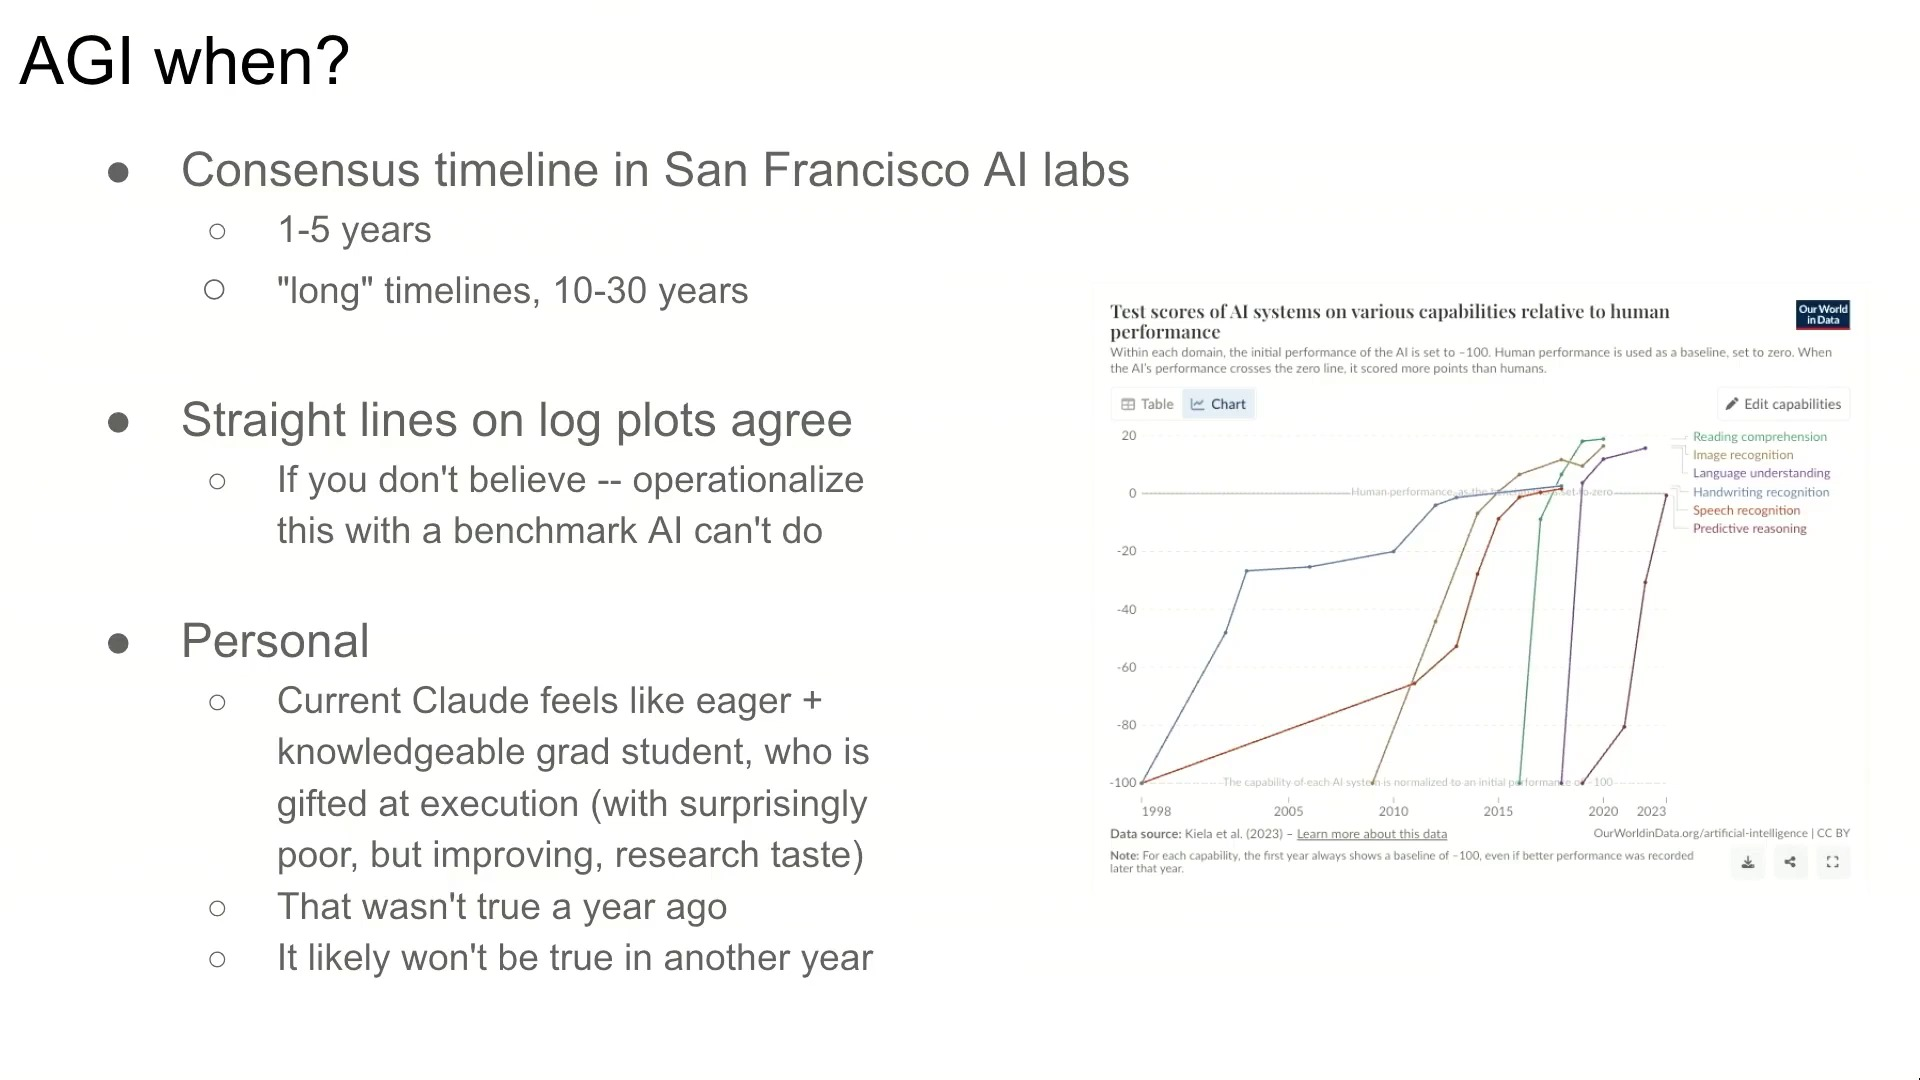
\includegraphics[width=0.92\textwidth]{figures/fig_10_sf_lab_timelines.jpg}
\caption{“AGI 何时到来？”：旧金山 AI 实验室的 1--5 年主流共识时间线、Our World in Data 多领域基准测试跨越人类水平线（0 分线）的加速曲线，以及讲者对当前 Claude 研究能力的定性评估\vtag}
\end{figure}
\srcnote{00:12:05--00:14:10}

Sohl-Dickstein 在上图中给出了三个层面的判断：
\begin{enumerate}
    \item \textbf{旧金山 AI 实验室的内部共识时间线（Consensus timeline in San Francisco AI labs）}：主流共识集中在 \textbf{1--5 年}；即便是在实验室内部自诩持有“漫长时间线（long timelines）”的怀疑派，其预测区间也仅仅是 \textbf{10--30 年}，几乎没有人认为需要五十年或一百年。
    \item \textbf{对数图上的直线全部指向同一结论（Straight lines on log plots agree）}：右侧嵌入的 Our World in Data 图表（数据源：Kiela et al., 2023）展示了 AI 系统在手写识别、语音识别、图像识别、阅读理解、语言理解与预测推理等不同能力维度上相对于人类表现（设为 $0$ 分基线，初始年份设为 $-100$）的追赶轨迹。1998 年启动的早期基准往往需要耗费 15--20 年才勉强触及人类水平线，而 2015--2020 年后设立的新兴高难度认知基准，几乎无一例外在发布后的短短数月到一两年内被近乎垂直的曲线一举击穿。讲者向所有怀疑者提出了一个科学可证伪性挑战：\textbf{“如果你不相信这一趋势，请给出一个具体的、可操作化的基准测试（operationalize this with a benchmark AI can't do），明确赌它在三年后依然无法被 AI 解决。”}
    \item \textbf{个人的一手科研体感（Personal experience）}：在日常合作中，当前的 Claude 感觉就像一位\textbf{“充满热情、知识面极广、在具体执行上极具天赋，但科研品味（Research Taste）出奇地差——尽管这种品味正在改善——的博士研究生”}。更重要的是，一年前它还完全不具备这种研究生级别的执行力，而再过一年，它在科研品味上的短板也极可能被补齐。
\end{enumerate}

\subsection{中场深度问答：科研品味、合成数据极限与世界模型}

在进入下半场行动建议之前，现场听众围绕“模型能否真正具备科学创造力与科研品味”展开了约 7 分钟的高质量交锋（对应视频 \texttt{00:14:15--00:20:55}）：

\begin{knowledgebox}{中场交锋精粹：AI 能否学会“科研品味”并突破训练数据天花板？}
\begin{enumerate}
    \item \textbf{问：科研品味（Research Taste）和提出真正新颖科学问题的能力，是否超出了现有强化学习（RL）与预训练的范畴？}
    
    \textbf{Sohl-Dickstein 答}：许多学者倾向于把“科研品味”神秘化。事实上，每当我们阅读一篇论文或审视一个实验构想并感叹“这是一个好想法”时，我们的大脑都在运行某种内部价值函数（Value Function）。只要人类能够事后分辨哪些研究路径产出了简洁、普适、可验证的成果，这种评判信号就是可形式化、可训练的。一年前人们还认为大模型只会机械背诵套路、绝不可能自主证明开放的 Erdős 数学难题；如今 27 个全自主求解已经证明，随着长程强化学习与推理搜索的深入，模型正在迅速内化对“什么是好证明、好方向”的直觉。

    \item \textbf{问：互联网人类文本已经接近枯竭，依靠模型生成合成数据（Synthetic Data）或自我博弈会不会导致模型坍缩或停留在已有知识边界内？}
    
    \textbf{Sohl-Dickstein 答}：不妨反观人类科学共同体自身——全人类并没有接收来自外星高等文明的“超人类预训练语料”。每一个人类婴儿降生时接收的都是有限的感官输入与前人留下的教材，但人类通过内部思考（如同思维链推理）、提出假说、向自然界做实验获取反馈以及多智能体之间的学术争鸣，持续不断地推高了整个人类的知识边界。同样地，当基础模型结合代码执行器、形式化验证器（如 Lean）与真实科学实验闭环时，它并不受限于静态网页语料的上界。

    \item \textbf{问：当前 LLM 在三维空间推理、物理直觉与具身交互（空间智能）上依然笨拙，这是否会拖慢 AGI 时间线？}
    
    \textbf{Sohl-Dickstein 答}：我完全同意当前模型在空间与多模态几何直觉上弱于纯符号与代码领域。但关键在于，绝大多数现代科学发现、数学推导、政策分析、软件研发乃至下一代 AI 架构设计本身，核心瓶颈都是\textbf{符号、逻辑与计算认知工作}，而非像灵长类动物那样在树林间敏捷跳跃。认知自动化的爆发并不需要等待机器人具备完美的手眼协调能力。
\end{enumerate}
\end{knowledgebox}

\subsection{本章小结}
本章梳理了短期 AGI 预期如何在一年内从受人嘲笑的“疯狂摘要”演变为英美政商高层与《经济学人》《纽约时报》的主流议题，解析了旧金山 AI 实验室内部“1--5 年主流共识、10--30 年长线派”的时间线分布及基准饱和曲线，并通过现场问答阐明了“科研品味可经由内部价值函数与环境反馈习得，纯认知自动化无需等待具身空间智能完全成熟”的核心逻辑。

\clearpage
\section{黄金窗口期的四项行动准则：当智力贡献只剩 1--5 年}

既然证据链与前沿实验室共识均指向未来 1--5 年内人类智力劳动范式的根本性重构，那么作为一名当下仍在高校或研究机构求学、执教的研究者，应当如何行动？Sohl-Dickstein 以一个直击灵魂的设问开启了报告的下半场：\textbf{“如果我只剩下 1--5 年的时间能够向世界做出独特的个人智力贡献，我现在最应该做什么？（I have 1-5 years to contribute intellectually to the world. What should I do?）”}并给出了四条环环相扣的行动准则。

\subsection{准则一：让项目周期短于指数特征时间尺度，践行《苦涩的教训》}

第一条准则聚焦于\textbf{如何选择科研课题与合作模式}（见下图）：优先选择雄心勃勃、目标高度聚焦、能够快速推进的协作项目（Prefer ambitious, targeted, \textit{fast} collaborations），绝不要在漫长、孤立、缺乏明确方向的慢速摸索中消耗宝贵窗口期。

\begin{figure}[H]
\centering
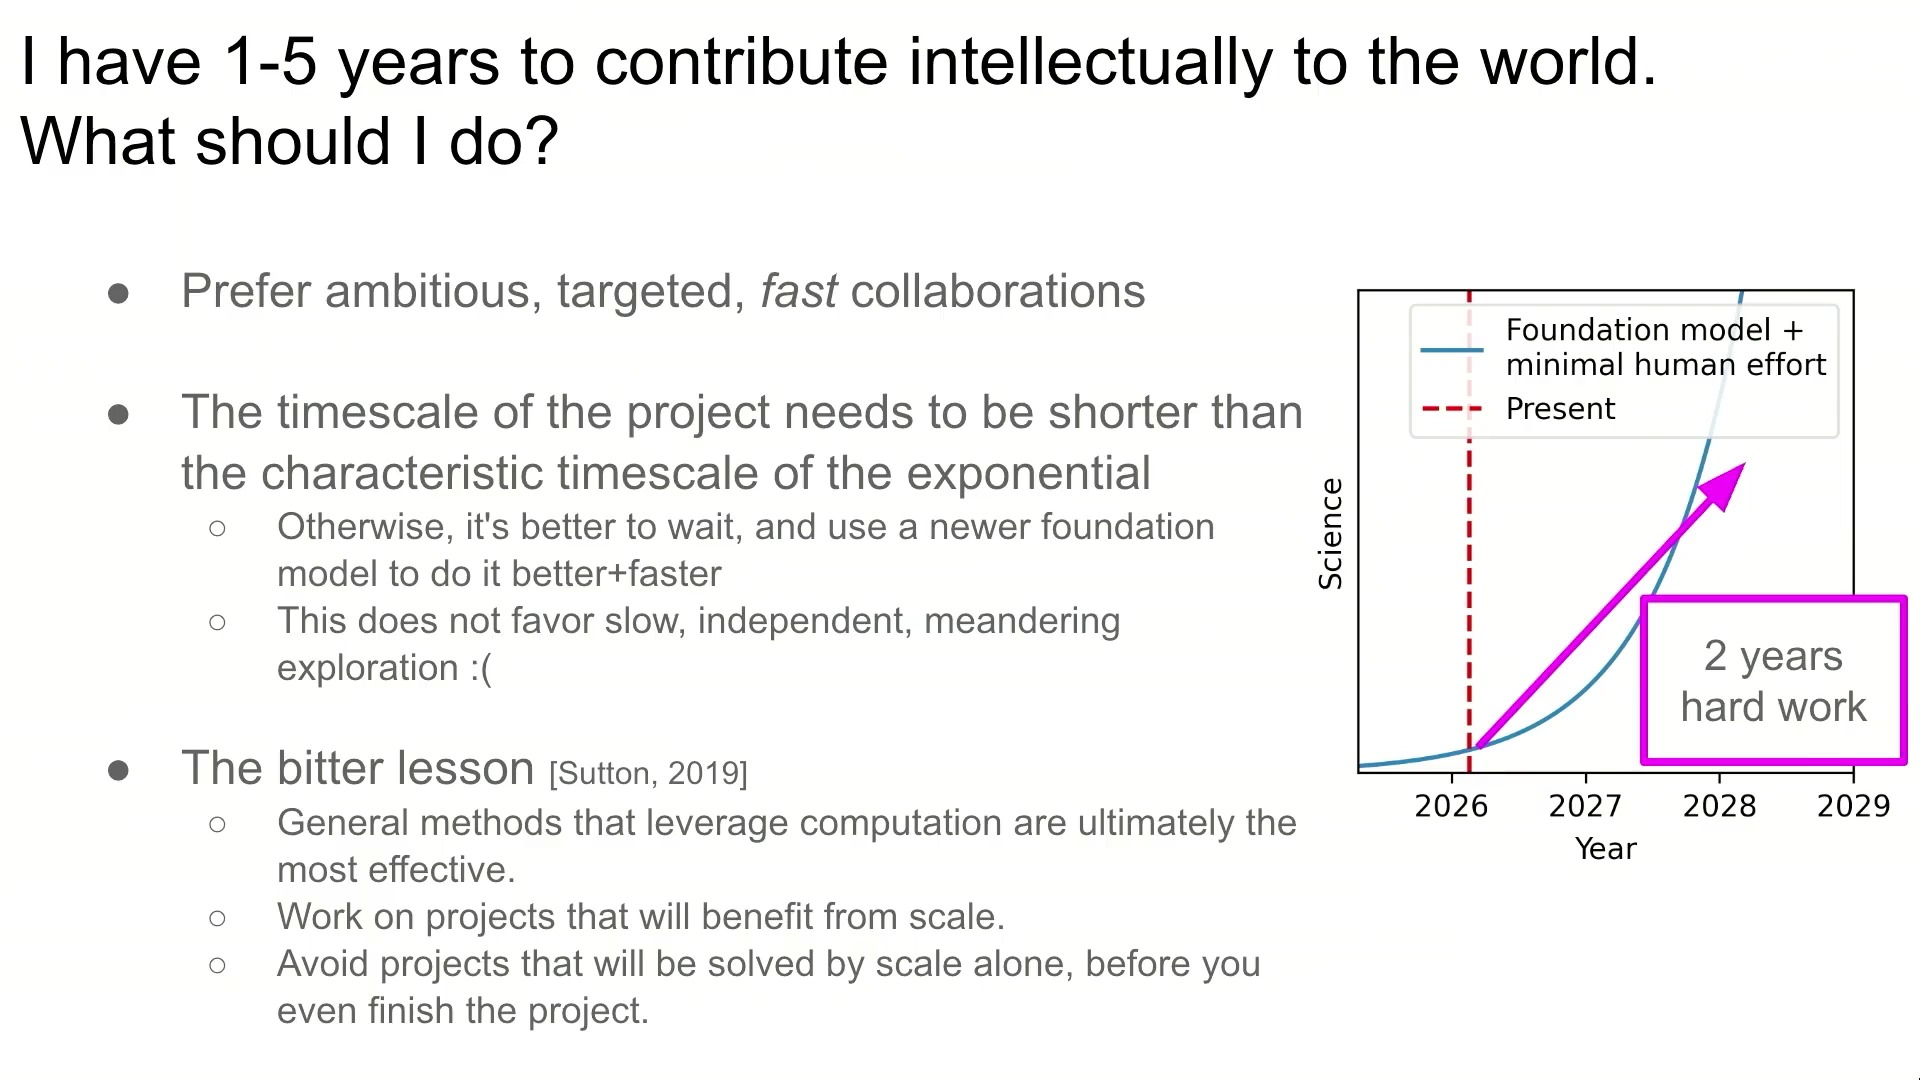
\includegraphics[width=0.92\textwidth]{figures/fig_11_project_timescale_bitter_lesson.jpg}
\caption{行动准则一：项目的完成时间尺度必须短于指数增长的特征时间尺度（右图对比了“苦干 2 年的线性推进”与“等待下一代基础模型 + 极少人工投入”的产出曲线），并遵循 Rich Sutton（2019）《苦涩的教训》\vtag}
\end{figure}
\srcnote{00:14:15--00:23:05}

为什么慢工出细活的传统个人探索模式在当下极其危险？讲者通过图右侧的“科学产出 vs.\ 年份（2026--2029）”示意图给出了严格的数学直觉：图中蓝色指数曲线代表“仅靠当时最新的基础模型 + 极少量人类介入（Foundation model + minimal human effort）”所能达到的科学水平；红色竖虚线代表当下（2026 年初）；而品红色粗箭头则代表一名研究者从今天立项、埋头苦干整整两年（2 years hard work）所取得的线性进展。可以看到，当这名研究者在 2028 年终于拼尽全力到达品红色箭头终点时，蓝色指数曲线早已在更早的时间点 effortlessly（毫不费力地）越过了同一高度。

将这一几何关系写为定量判据，假设基础模型在目标领域的能力随时间 $t$ 按年化倍增因子 $r$（例如算力 $r \approx 4.7\,\text{yr}^{-1}$，或任务时长每 $T_{1/2} \approx 0.58\text{ yr}$ 翻一番）呈指数增长 $S(t) = S_0 e^{t / \tau_{\text{exp}}}$，则任何人类主导科研项目的计划周期 $\tau_{\text{project}}$ 必须满足特征时间尺度不等式：

\[
\tau_{\text{project}} < \tau_{\text{exp}} = \frac{1}{\ln r} = \frac{T_{1/2}}{\ln 2}
\]

式中各参数的含义如下：
\begin{itemize}
    \item $\tau_{\text{project}}$：从课题立项、实验攻关到成果发表落地所需的项目总时间跨度；
    \item $\tau_{\text{exp}}$：底层基础模型能力指数增长的特征时间尺度（Characteristic timescale of the exponential，$e$ 折时间）；
    \item $r$：能力指标的年化增长倍数；
    \item $T_{1/2}$：基础模型有效任务跨度或推理能力的倍增周期（Doubling time）。
\end{itemize}

\begin{importantbox}{核心方法论：指数时代的《苦涩的教训》（The Bitter Lesson）双向推论}
强化学习先驱 Rich Sutton 在 2019 年发表的短文《苦涩的教训》（\textit{The Bitter Lesson}）指出：回顾过去七十年的 AI 研究史，凡是试图把人类专家的领域技巧硬编码进系统的精巧方法，最终无一例外都被“能够直接利用通用算力规模扩张（General methods that leverage computation）”的简单方法彻底击败。Sohl-Dickstein 将这一教训提炼为当下选题的\textbf{一正一反两条铁律}：
\begin{enumerate}
    \item \textbf{正向借力（Ride the scale）}：致力于那些随着底层模型算力与智能水平跃升而水涨船高、直接受益于规模扩张（Benefit from scale）的架构、评测、科学应用或治理框架；
    \item \textbf{反向避坑（Avoid scale-doomed work）}：坚决避开那些“还没等你把这个两年期项目做完，下一代大模型单靠规模增长（Solved by scale alone）就会顺手彻底解决”的修补性课题。
\end{enumerate}
\end{importantbox}

\subsection{准则二：拥抱“反人体工学”的新工具，把做 PI 与写 Prompt 融会贯通}

第二条准则聚焦于\textbf{日常科研工作流的彻底升级}（见下图）：立即学习并高频使用最新的基础模型工具，哪怕它们今天用起来依然别扭、充满摩擦（Non-ergonomic）。

\begin{figure}[H]
\centering
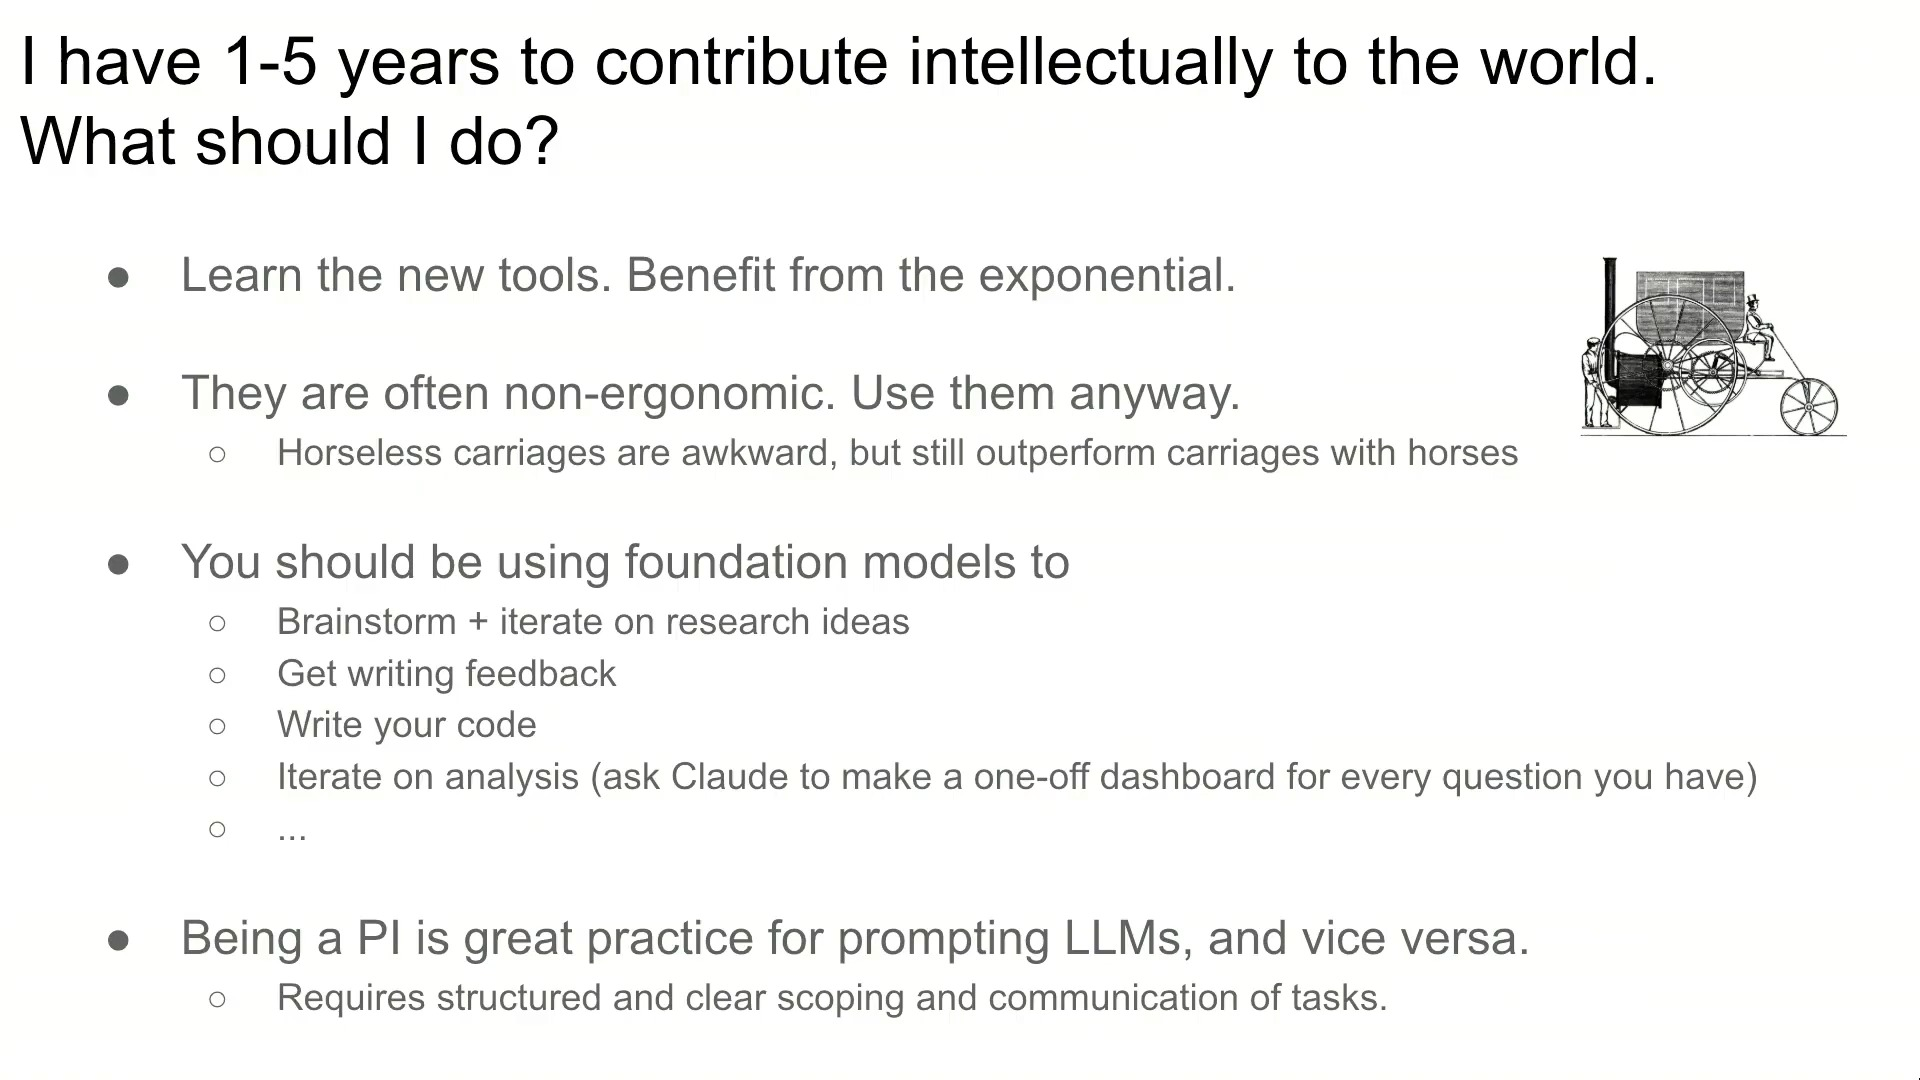
\includegraphics[width=0.92\textwidth]{figures/fig_12_horseless_carriage_tools.jpg}
\caption{行动准则二：十九世纪末“无马马车（Horseless Carriage）”的隐喻、基础模型在科研全流程中的四类用法，以及“做课题组导师（PI）与提示工程（Prompting LLMs）互为最佳训练”\vtag}
\end{figure}
\srcnote{00:23:05--00:24:35}

讲者在幻灯片右上角放了一幅十九世纪末早期蒸汽/内燃机“无马马车（Horseless carriage）”的版画：早期的汽车没有方向盘、直接照搬马车车厢结构，不仅噪音震耳欲聋、故障频发，操控体验更是远不如一匹训练有素的温顺老马。许多习惯了传统马车的车夫在试驾一次后便嘲笑它“根本不好用”。然而，无马马车背后的动力来自热力学与工业指数增长，哪怕形态再笨拙，它也迅速在速度与载荷上全面碾压了生物马匹。今天的大语言模型与编程 Agent 正是科研界的“无马马车”。

具体而言，讲者建议每位研究者立即在以下四个环节重度使用基础模型：
\begin{itemize}
    \item \textbf{头脑风暴与课题迭代（Brainstorm + iterate on research ideas）}：将模型作为全天候的跨学科讨论伙伴，快速排查文献盲区与反例。
    \item \textbf{获取论文写作反馈（Get writing feedback）}：讲者在此特别强调了一条红线——\textbf{不要让大模型替你写初稿（Don't have it write your first draft）}，因为亲手组织语言的过程就是理清科学逻辑的过程；但初稿完成后，让大模型扮演苛刻的审稿人来挑刺结构漏洞与表述歧义，效率极高。
    \item \textbf{编写全部实验代码（Write your code）}：将精力从语法调试转向实验设计与结果验证。
    \item \textbf{高频迭代数据分析——为每一个问题定制一次性交互看板（One-off dashboard for every question）}：过去为了看清高维实验数据中的某个切片，写一套可视化界面往往耗时数天，不划算；而现在，每当你脑中闪过一个探索性问题，都可以直接要求 Claude 在几分钟内为你生成一个专属的交互式分析看板（Dashboard），用完即弃。
\end{itemize}

更有趣的是，讲者指出：\textbf{“担任课题组负责人（Being a PI）是练习给大模型写 Prompt 的绝佳训练，反之亦然。”}因为这两件事的核心能力完全同构——都要求你把一个模糊宏大的科学愿景，清晰、结构化地拆解（Structured and clear scoping）为边界明确、上下文自洽、验证标准清晰的子任务，并准确传达给执行者（无论是人类研究生还是 Claude Agent）。

\subsection{准则三：破除认知失调，重构高基线颠覆风险下的职业权衡}

第三条准则直指学术界普遍存在的\textbf{言行割裂（Cognitive Dissonance）}。

\begin{figure}[H]
\centering
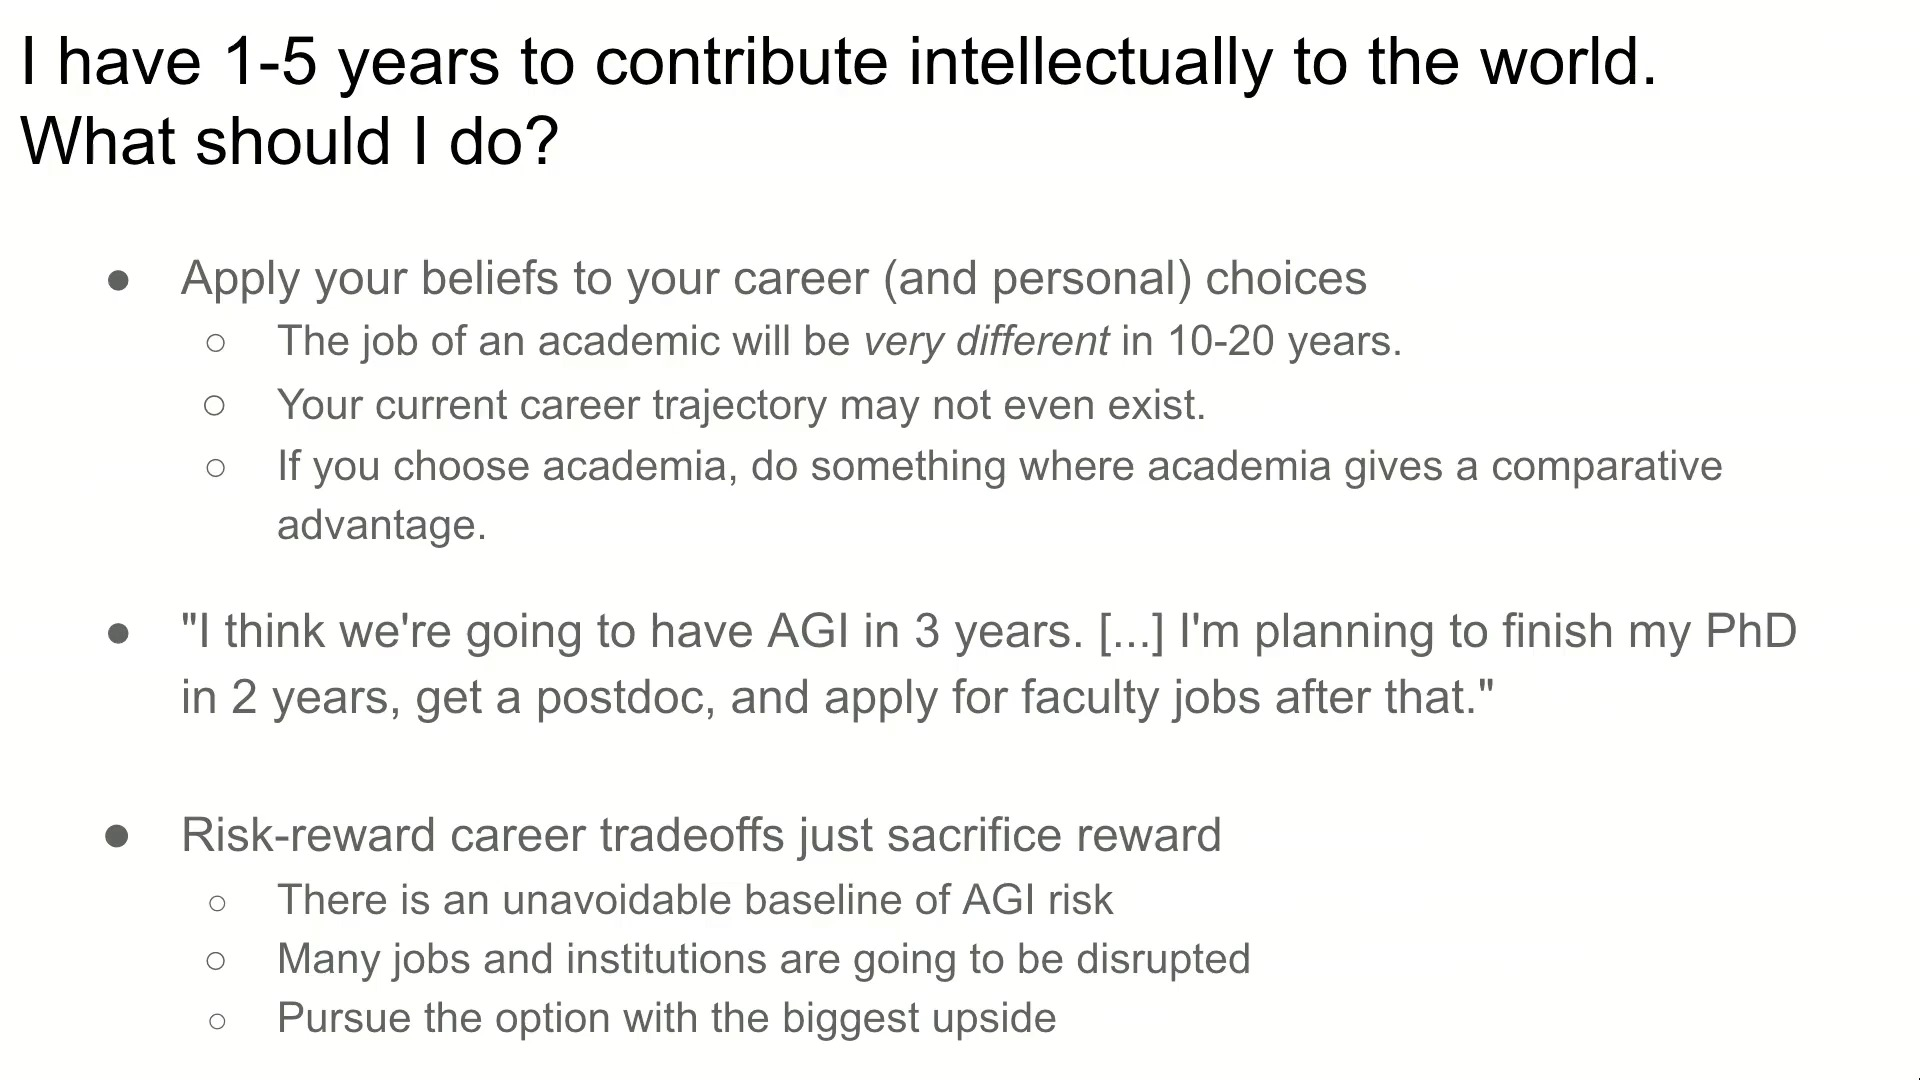
\includegraphics[width=0.92\textwidth]{figures/fig_13_career_risk_reward.jpg}
\caption{行动准则三：将你对 AGI 的真实判断切实应用到个人职业决策中，破除“相信 3 年内实现 AGI 却按部就班规划博士—博后—教职”的认知失调\vtag}
\end{figure}
\srcnote{00:24:35--00:26:10}

Sohl-Dickstein 复述了他在与顶尖高校博士生交流时听到过无数次的一段标准对话（见上图第二条）：
\begin{quote}
“我认为我们将在 3 年内迎来 AGI。……至于我的个人规划，我打算再用 2 年读完博士，然后去做一期博士后，之后再申请高校教职（Faculty jobs）。”
\end{quote}
现场听众闻言哄堂大笑。为什么这句话如此荒诞？因为“读完博士 $\to$ 2--3 年博后 $\to$ 5--6 年助理教授冲击终身教职（Tenure）”是一套为\textbf{未来 10--20 年社会与学术体制保持基本稳定}而设计的长周期投资方案。如果你真诚地认为未来 3--5 年内机器将在绝大部分认知任务上超越人类，那么 10--20 年后的大学教授职位（如果还存在的话）其工作内容也将与今天面目全非。

\begin{warningbox}{职业决策误区：当存在高基线颠覆风险时，“求稳”只会白白牺牲上限}
在和平稳定的年代，年轻学者常在“稳妥但影响力平庸的保底方向（Safe option）”与“高风险但一旦成功就能改变领域的大胆方向（Ambitious option）”之间做风险收益权衡（Risk-reward tradeoff）。但讲者指出，在 AGI 即将带来全局性洗牌的时代，整个社会存在一个\textbf{不可避免的高基线颠覆风险（Unavoidable baseline of AGI risk）}——无论你选哪条路，传统的职业晋升阶梯与按部就班的岗位都有极高概率被重构。既然“保守选项”根本无法为你买来真正的安全感，那么为了所谓求稳而放弃高上限课题，就等于\textbf{白白牺牲了回报上限却没有降低风险（Risk-reward career tradeoffs just sacrifice reward）}。此时唯一理性的策略是：\textbf{直接追求潜在正面影响力上限最高（Biggest upside）的选项}；如果你依然选择留在高校，请务必利用高校独有的比较优势（Comparative advantage，如学术独立性、社会公信力与长远公共利益视角）去做工业界无法或不愿做的事。
\end{warningbox}

\subsection{准则四：选择能够偏转长期轨迹而非制造瞬态扰动的课题}

第四条准则从时间积分的角度定义了什么才是真正有价值的科学贡献（见下图）。

\begin{figure}[H]
\centering
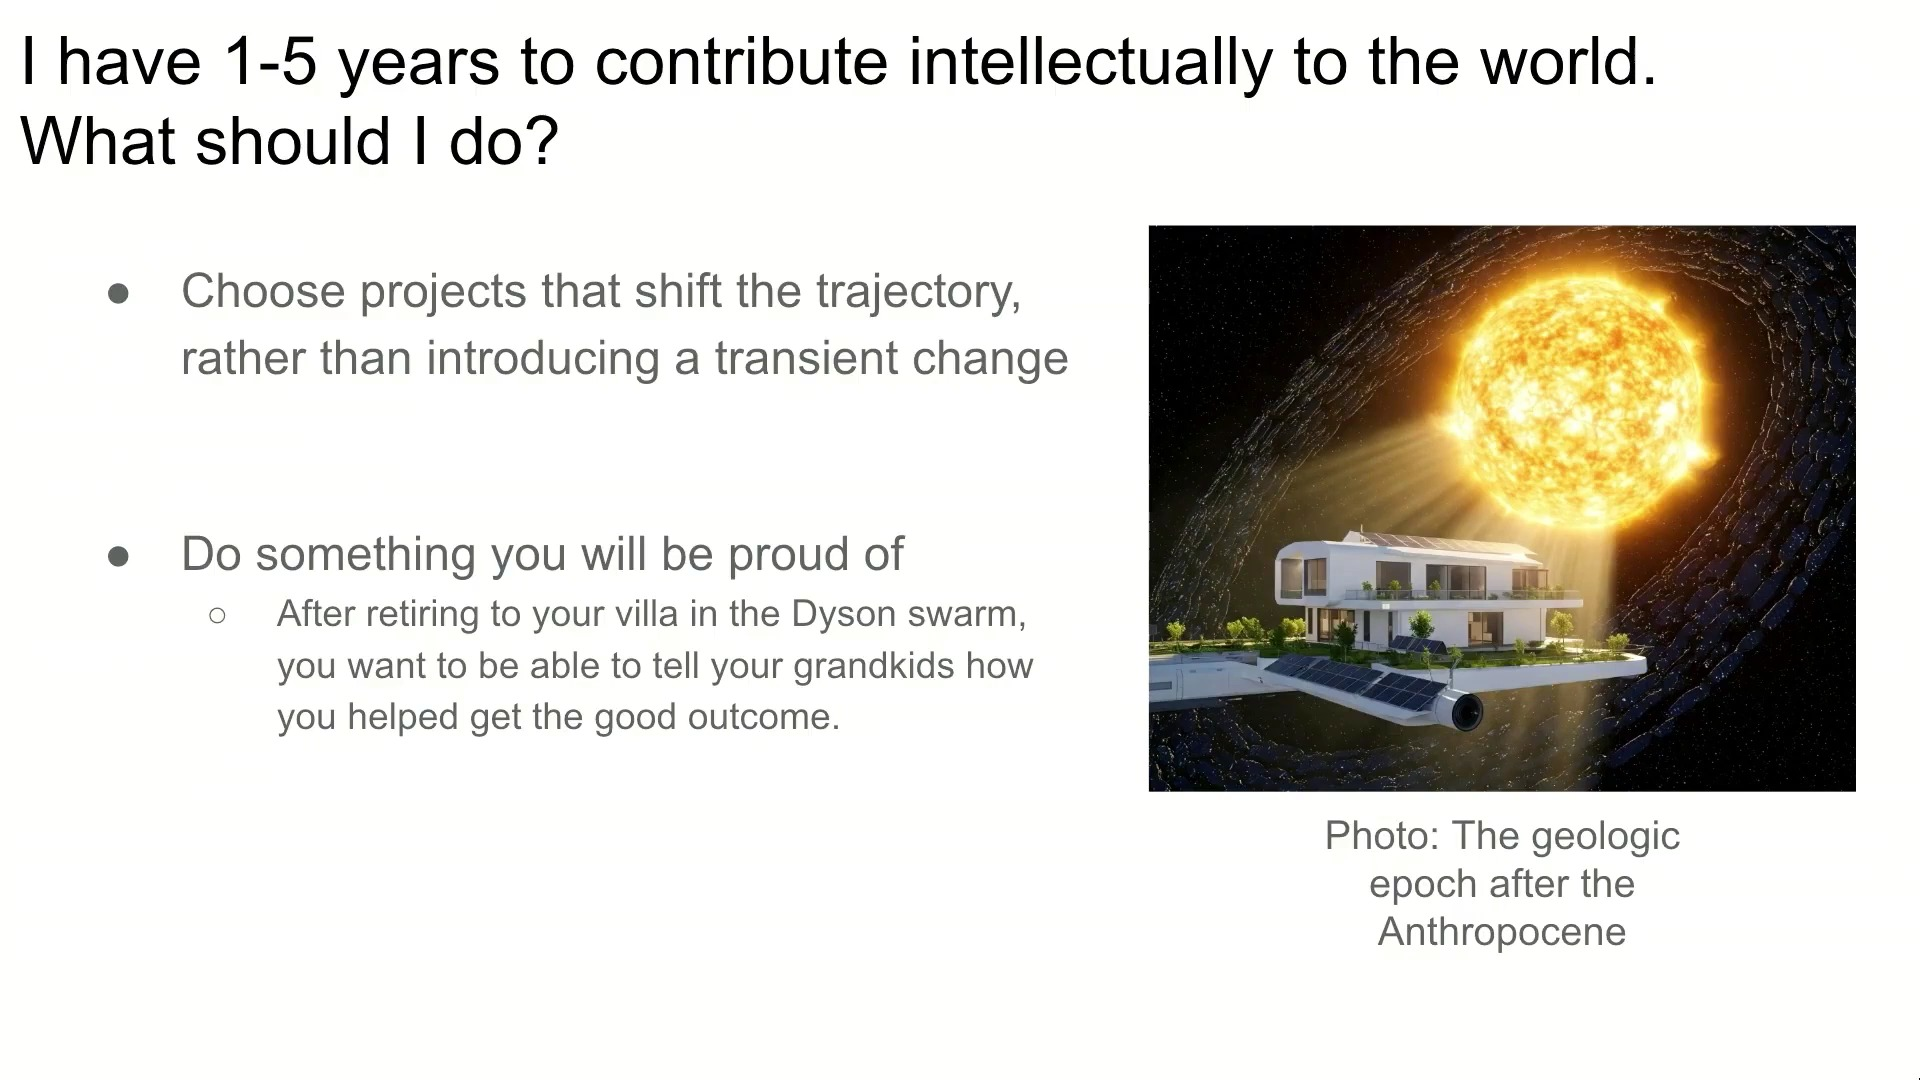
\includegraphics[width=0.92\textwidth]{figures/fig_14_trajectory_shift_dyson.jpg}
\caption{行动准则四：选择能够长期偏转演化轨迹（Shift the trajectory）而非仅引入瞬态变化（Transient change）的课题；右图为“人类世之后的下一个地质纪元”——环绕恒星的戴森云（Dyson Swarm）栖息地畅想\vtag}
\end{figure}
\srcnote{00:26:10--00:27:25}

在动力学系统中，对一个系统的干预分为两类：
\begin{itemize}
    \item \textbf{瞬态扰动（Transient change）}：例如把某个通用大模型基准测试的刷榜精度提高 $0.5\%$，或者把某个已经在工业界路线图上的工程优化提前两个月做出来。无论你今天做不做这件事，三个月后下一代模型都会自然覆盖这一进展，十年后回看，历史轨迹没有发生任何丝毫改变。
    \item \textbf{轨迹偏转（Shift the trajectory）}：改变系统的初始方向角、游戏规则、安全边界、评测标准或制度规范。哪怕初始偏转角只有 $1^{\circ}$，在随后的指数扩张中也会导向截然不同的终局。
\end{itemize}

讲者指着右侧那幅环绕恒星建造的“戴森云（Dyson Swarm，将恒星辐射能量大规模捕获并转化为计算与生存空间的太空巨型结构）”概念图幽默地说道：“这幅照片展示的是人类世之后的下一个地质纪元。当你未来退休、住进戴森云里的花园别墅时，你希望能够骄傲地向孙辈讲述：在当年那场决定人类命运的转折关头，我究竟做了什么帮助人类迎来了美好的结局（helped get the good outcome）。”

\subsection{本章小结}
本章系统阐述了面向 1--5 年智力贡献窗口期的四项行动准则：（1）项目周期 $\tau_{\text{project}}$ 必须短于指数增长特征尺度 $\tau_{\text{exp}}$，并遵循《苦涩的教训》借力规模扩张、避开易被算力顺手抹平的课题；（2）跨越“无马马车”的初期不适，用大模型重塑头脑风暴、审稿润色（坚持手写初稿）、编码与一次性看板分析，发挥做 PI 与写 Prompt 的同构优势；（3）消除认知失调，在高基线颠覆风险下果断追求最高上限；（4）放弃瞬态刷榜，专注于能产生长期路径偏转（Shift the trajectory）的工作。

\clearpage
\section{指数早期的巨大杠杆：为什么个体选择能决定未来技术树}

面对庞大的科技巨头与百亿美元级的数据中心集群，个体研究者很容易陷入一种无力感，认为 AI 的演进是一列早已锁死轨道、不受个人意志转移的历史列车。Sohl-Dickstein 在报告第五部分明确反驳道：\textbf{“认为 AI 是超出个人控制之外的自发过程——这是彻底错误的（This is false）。我们目前依然处于指数增长的极早期阶段，你个人对 AI 的未来拥有巨大的权力与杠杆（Immense power and leverage）。”}

\subsection{Epoch AI 2030 算力扩展约束：为什么今天仍是“指数极早期”？}

为了证明“现在依然是极早期”，讲者引用了研究机构 Epoch AI 发布的《2030 年训练运行扩展约束》（\textit{Constraints to scaling training runs by 2030}）定量评估报告（见下图）。

\begin{figure}[H]
\centering
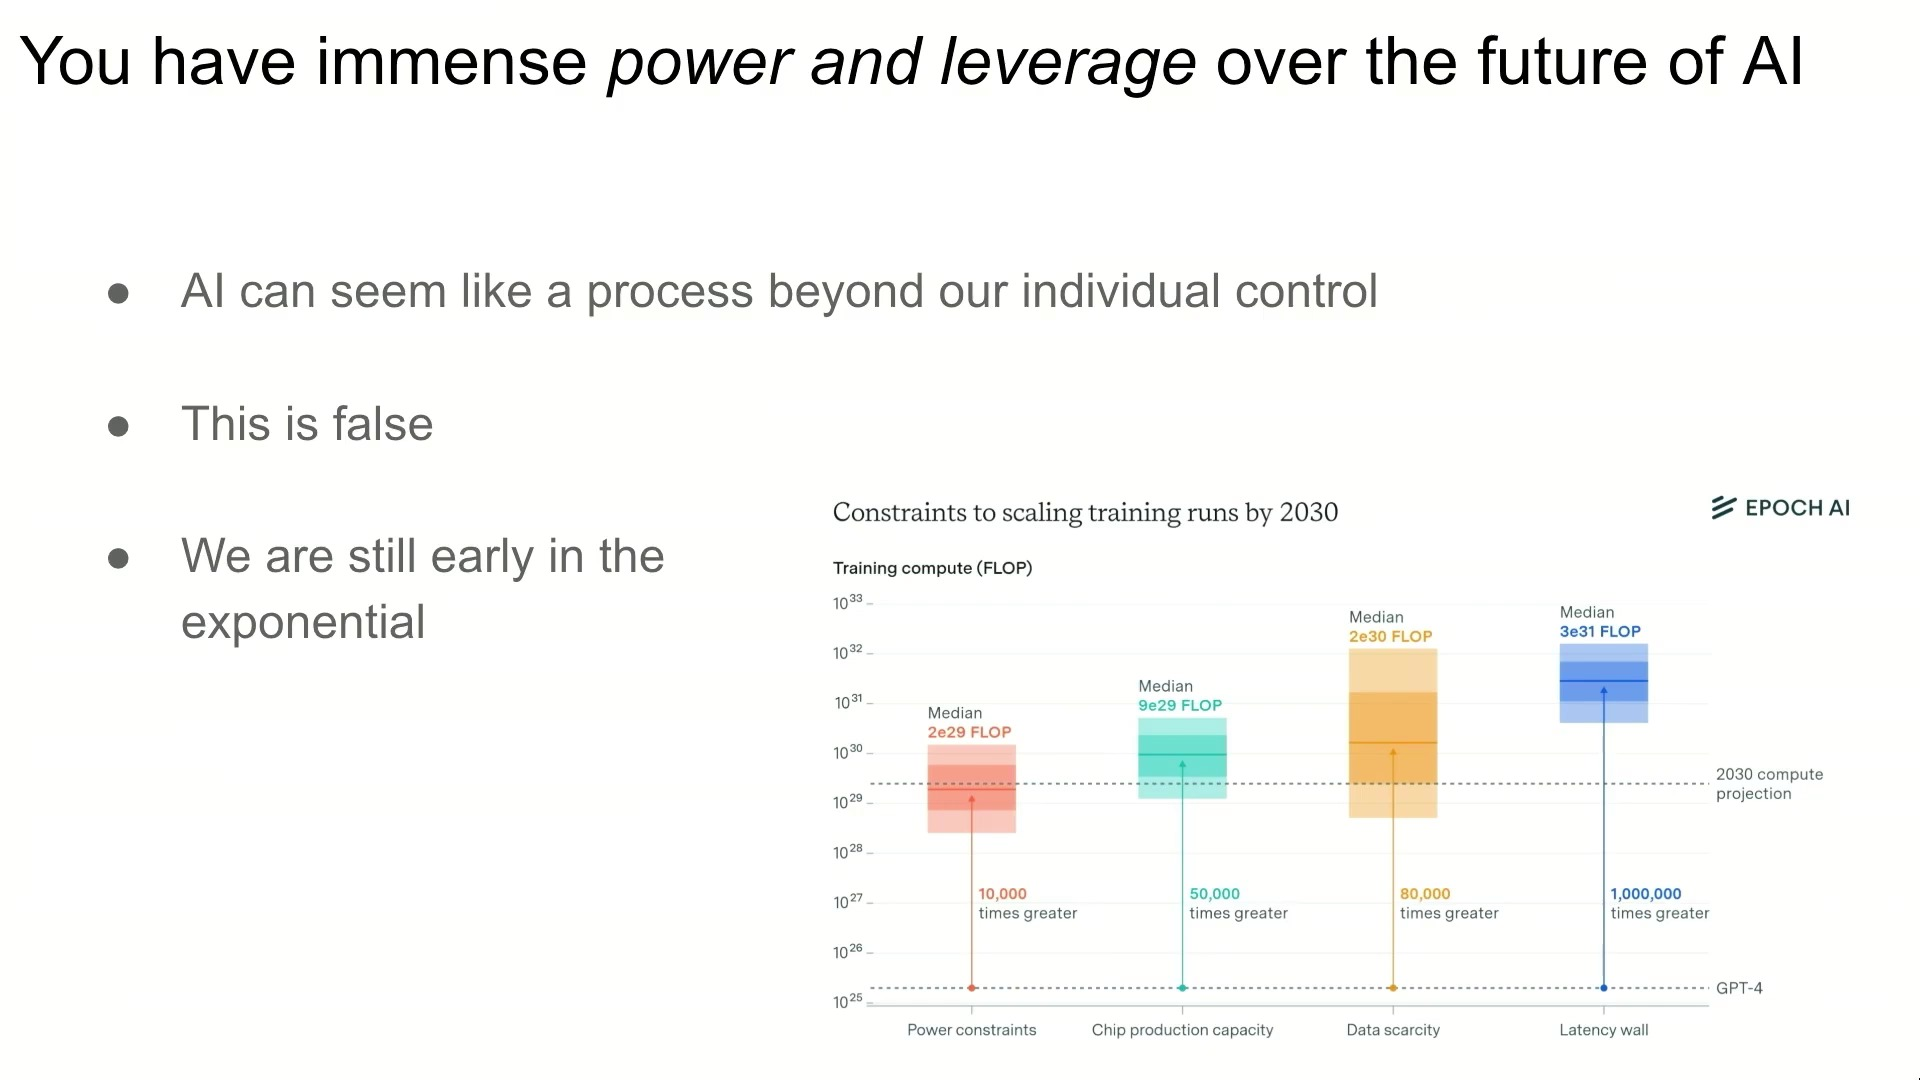
\includegraphics[width=0.92\textwidth]{figures/fig_15_epoch_scaling_2030.jpg}
\caption{Epoch AI 对 2030 年前沿训练运行算力上限的四大瓶颈测算：即便受最严苛的电力供应（Power constraints）限制，2030 年单次训练算力中位数预测（$2\times 10^{29}\text{ FLOP}$）仍比 GPT-4 基线高出 10,000 倍\vtag}
\end{figure}
\srcnote{00:27:25--00:28:40}

Epoch AI 团队深入核算了限制大模型训练算力继续扩张的四道硬性物理与工业瓶颈，并以 GPT-4 的训练算力（约 $2\times 10^{25}\text{ FLOP}$，图中底部虚线）为基准，测算了到 2030 年每一道瓶颈所允许的最大单次训练算力中位数（Median）：
\begin{enumerate}
    \item \textbf{电力供应约束（Power constraints）}：中位数上限为 \textbf{$2\times 10^{29}\text{ FLOP}$}，即比 GPT-4 大 \textbf{10,000 倍（一万倍）}；
    \item \textbf{芯片制造产能（Chip production capacity）}：中位数上限为 \textbf{$9\times 10^{29}\text{ FLOP}$}，比 GPT-4 大 \textbf{50,000 倍（五万倍）}；
    \item \textbf{高质量数据稀缺性（Data scarcity）}：中位数上限为 \textbf{$2\times 10^{30}\text{ FLOP}$}，比 GPT-4 大 \textbf{80,000 倍（八万倍）}；
    \item \textbf{通信延迟墙（Latency wall）}：中位数上限为 \textbf{$3\times 10^{31}\text{ FLOP}$}，比 GPT-4 大 \textbf{1,000,000 倍（一百万倍）}。
\end{enumerate}

取上述四道约束中最严苛的短板（电力约束），到 2030 年单次训练运行的算力规模依然将达到今天的 \textbf{10,000 倍}左右。这意味着，如果把 2030 年的 AI 生态比作一棵参天巨树，那么今天的全部大模型产业仅仅是刚刚破土而出、不到其万分之一体量的嫩芽。而在任何指数生长过程的极早期，对幼苗生长方向的微小拨动，都会在树冠层产生数以百米计的位移。

\subsection{九大历史先例：指数增长早期的微小决策如何锁定百年格局}

为了具象化展示“早期微小干预 = 长期巨大后果（Small choices early in exponential growth have huge consequences）”，讲者一口气列举了科技史、医学史与制度史上的九个经典案例（见下图与随后的解析表）。

\begin{figure}[H]
\centering
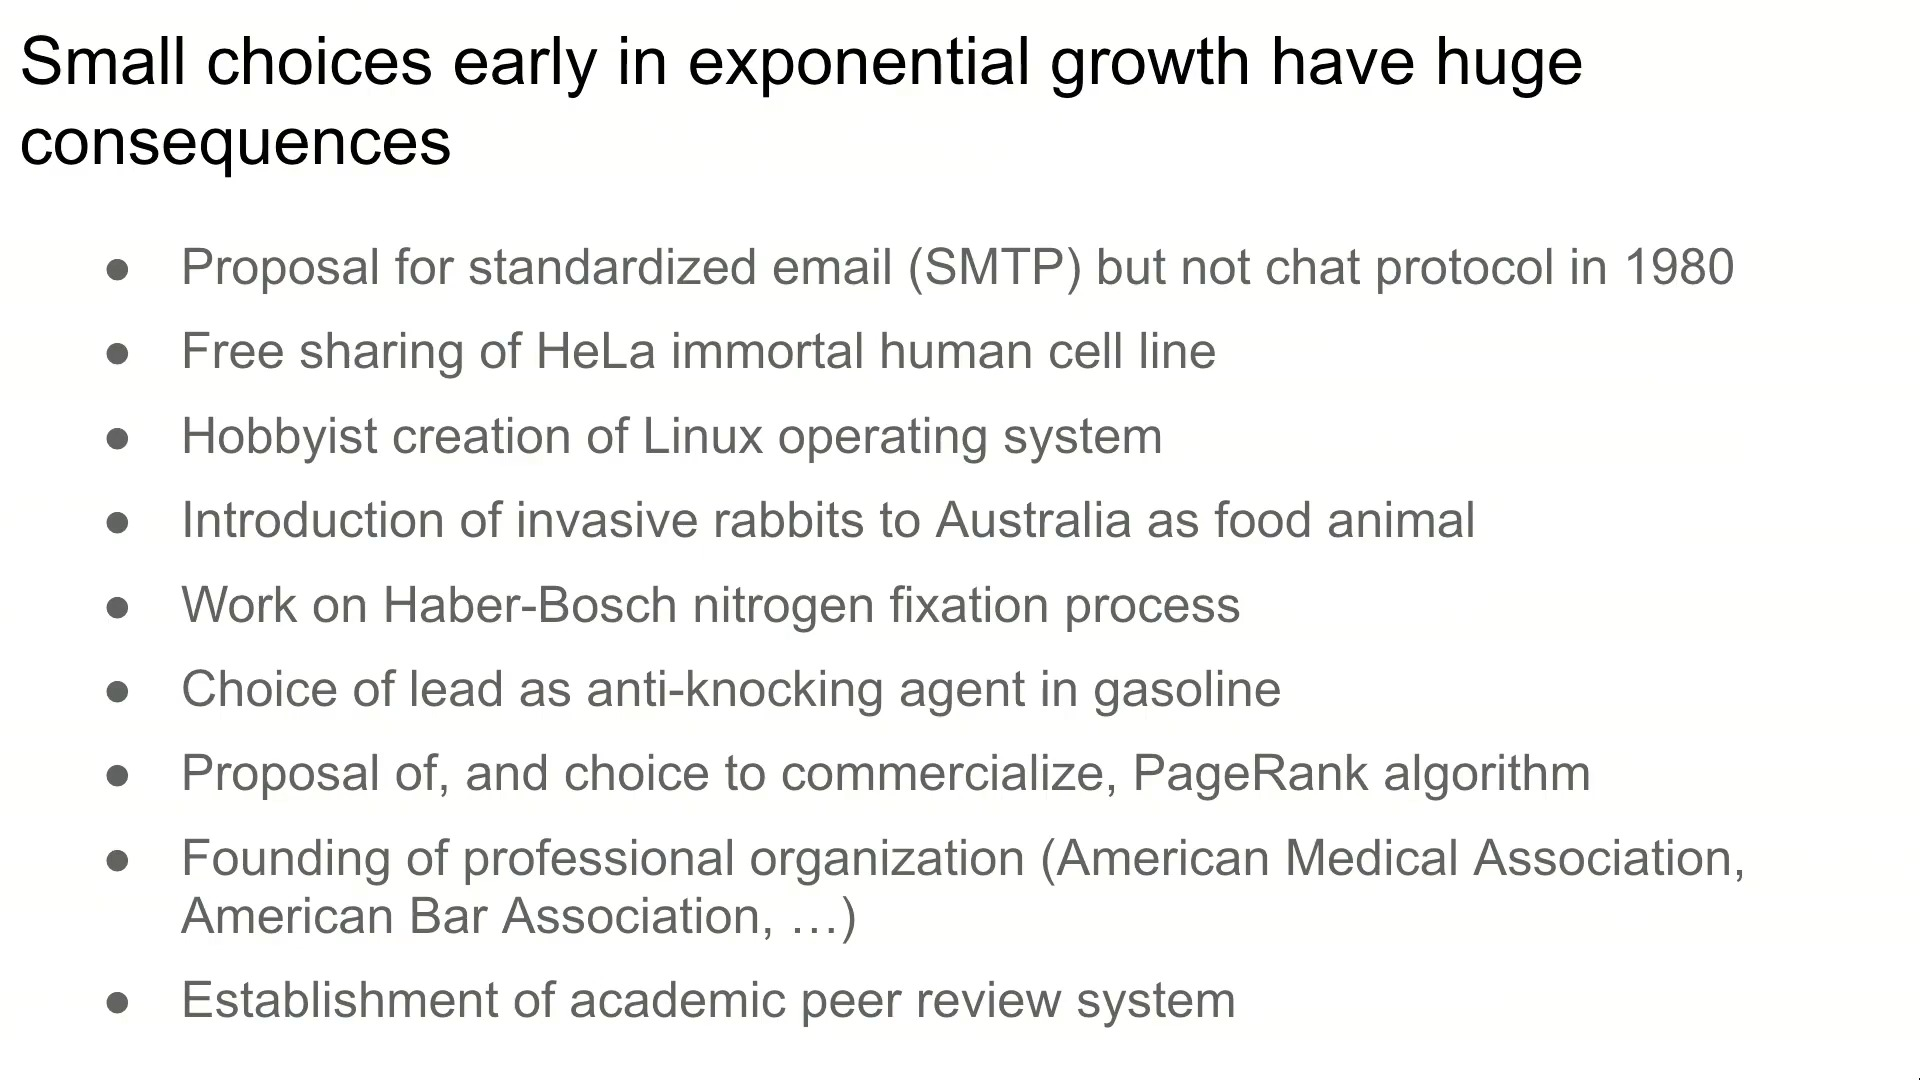
\includegraphics[width=0.92\textwidth]{figures/fig_16_historical_interventions.jpg}
\caption{历史实证：在指数增长早期做出的微小个人或小组决策（从 1980 年 SMTP 协议、HeLa 细胞免费共享、Linux 到同行评审制度），如何在数十年后深刻锁定全球技术与社会格局\vtag}
\end{figure}
\srcnote{00:28:40--00:31:00}

\begin{table}[H]
\centering
\small
\caption{指数增长早期微小决策产生巨大路径依赖的九大历史案例解析}
\begin{tabular}{p{3.4cm}p{4.6cm}p{5.6cm}}
\toprule
\textbf{历史案例与时间节点} & \textbf{指数早期的微小介入动作} & \textbf{经指数放大后的长期锁定后果} \\
\midrule
1.\ 1980 年电子邮件协议（SMTP）vs.\ 聊天协议 & Jon Postel 等极少数先驱在 1980 年起草并推广了跨机构开放电子邮件标准（SMTP），但当时无人替即时通讯（Chat）制定具备同等地位的去中心化通用标准 & 四十多年后的今天，全球任何人仍可跨服务商自由收发邮件，而即时通讯却彻底割裂为微信、WhatsApp、Slack、iMessage 等互不相通的封闭孤岛 \\
2.\ HeLa 永生人类细胞系的免费共享 & 1951 年 George Gey 实验室分离出首株人类永生细胞系 HeLa 后，决定不申请专利垄断，而是亲自带着试管免费分发给全球同行 & 直接催生了现代细胞生物学、脊髓灰质炎疫苗研发与生物医药产业的标准化实验基石（同时也暴露了早期知情同意伦理的缺失） \\
3.\ 业余爱好者创建 Linux 操作系统 & 1991 年芬兰大学生 Linus Torvalds 作为个人业余爱好开发内核并选用开源协议发布 & 如今支撑起全球绝大多数云服务器、超级计算机、安卓移动设备以及全部 AI 训练集群的底层操作系统底座 \\
4.\ 澳洲引入欧洲野兔作为食用动物 & 1859 年庄园主 Thomas Austin 仅为打猎与食用乐趣，将 24 只野兔释放到澳大利亚本土 & 缺乏天敌的野兔呈指数级繁殖至数亿只，酿成澳洲现代史上最严重的陆地生态崩溃与水土流失灾难 \\
5.\ 哈伯-博施（Haber-Bosch）固氮工艺 & 20 世纪初 Fritz Haber 与 Carl Bosch 攻克高温高压催化合成氨技术 & 人工合成化肥养活了当今地球约一半的人口（数十亿人），同时彻底改变了全球氮循环与现代炸药工业 \\
6.\ 选用四乙基铅作为汽油抗爆剂 & 1920 年代工程师 Thomas Midgley Jr.\ 在明知乙醇等无毒替代品可用的情况下，为追求专利利润选择向汽油添加四乙基铅 & 导致全球大气与土壤持续数十年的重金属铅污染，造成整整几代人智力受损与暴力犯罪率异常攀升 \\
7.\ PageRank 算法的提出与商业化选择 & 斯坦福博士生 Page 与 Brin 提出网页链接排序算法，并最终选择以“关键词竞价广告”而非学术订阅模式将其商业化 & 不仅塑造了现代互联网的信息检索入口，更将整个数字经济的商业模式锁定在“注意力捕获与广告变现”轨道上 \\
8.\ 专业行业协会（AMA / ABA）的创立 & 19 世纪中后期一小群医师与律师自发成立美国医学会（AMA）与美国律师协会（ABA） & 确立了延续百年的现代医师/律师执业资格审查、医学院认证体系与行业自律规范 \\
9.\ 学术同行评审（Peer Review）制度的确立 & 二战后（尤其 1960--1970 年代）部分期刊编辑部逐步推广外审专家匿名评审制度 & 并非自古有之的天然法则，却在随后半个世纪彻底定义了全球科学共同体的经费分配、职称晋升与知识认证标准 \\
\bottomrule
\end{tabular}
\end{table}

\subsection{个体撬动 AI 技术树的五个支点与个人智力回报曲线}

对比上述九个案例，今天的 AI 领域正处于完全相同的“规则未定、万倍扩张前夜”状态。每一位一线研究者在日常工作中的微小选择，都在实质性地修剪和引导未来的 AI 技术树（Tech Tree）：

\begin{figure}[H]
\centering
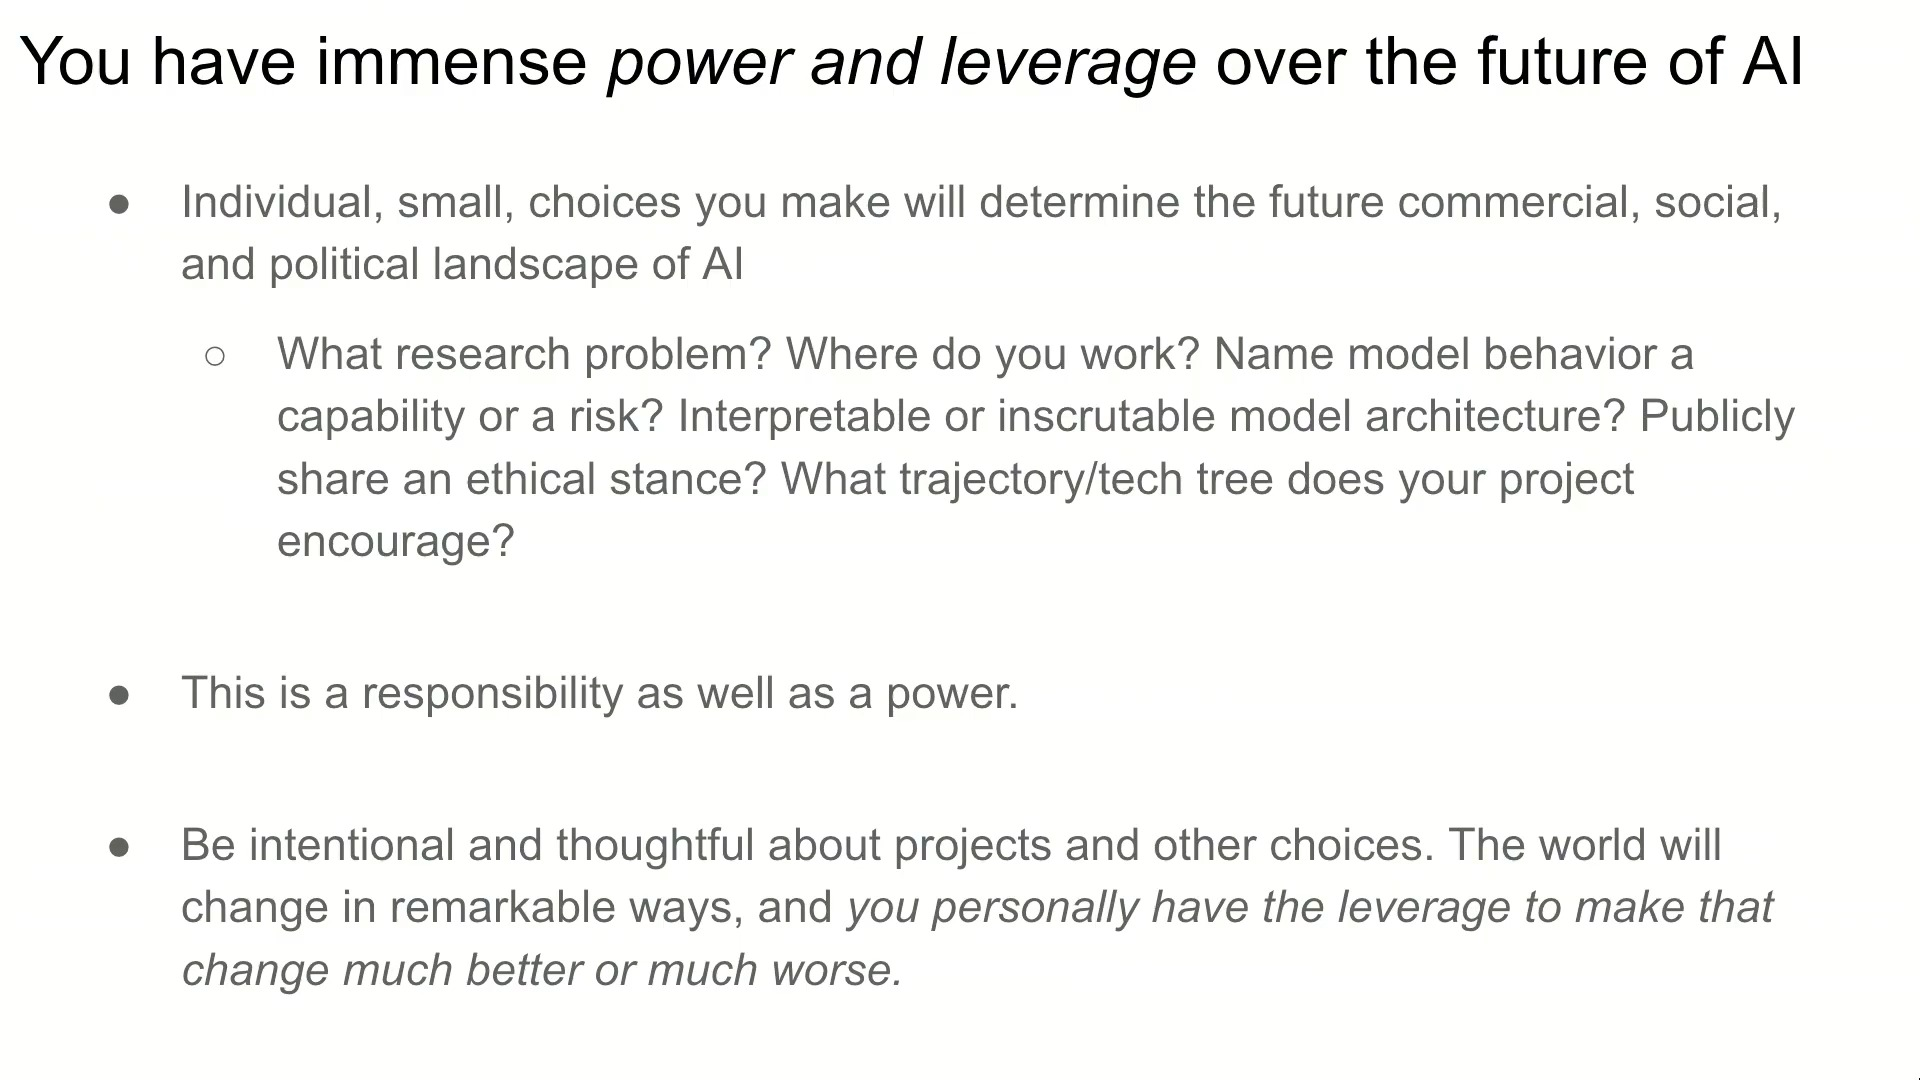
\includegraphics[width=0.92\textwidth]{figures/fig_17_tech_tree_leverage.jpg}
\caption{个体研究者决定未来 AI 商业、社会与政治格局的五个具体支点：选题、就职去向、将模型新行为命名为“能力”还是“风险”、架构透明度取向与公开伦理表态\vtag}
\end{figure}
\srcnote{00:31:00--00:31:55}

如上图所示，Sohl-Dickstein 点出了五个看似不起眼、实则具有巨大路径锁定效应的个人选择：
\begin{itemize}
    \item \textbf{你选择研究什么问题（What research problem?）}：你发表的基准与工具会吸引成百上千的后续跟进者；
    \item \textbf{你选择在哪里工作（Where do you work?）}：顶尖人才的用脚投票直接决定了哪家实验室、哪种安全文化能够胜出；
    \item \textbf{命名框架：将某种模型行为称为“能力”还是“风险”（Name model behavior a capability or a risk?）}：当你首次观察到模型出现某种新奇涌现行为时，如果你在开山论文中将其包装为炫酷的“自主规划能力（Capability）”，全行业就会竞相刷榜放大它；反之，如果你将其精准定义为“欺骗性奖励黑客风险（Risk）”，后续研究者就会围绕如何检测并抑制它展开攻关；
    \item \textbf{推进可解释架构还是黑箱架构（Interpretable or inscrutable model architecture?）}：架构层面的微小归纳偏置差异，决定了未来系统是否可审计；
    \item \textbf{是否公开分享你的伦理与安全立场（Publicly share an ethical stance?）}：打破沉默能够迅速改变同行群体的规范预期。
\end{itemize}

\begin{figure}[H]
\centering
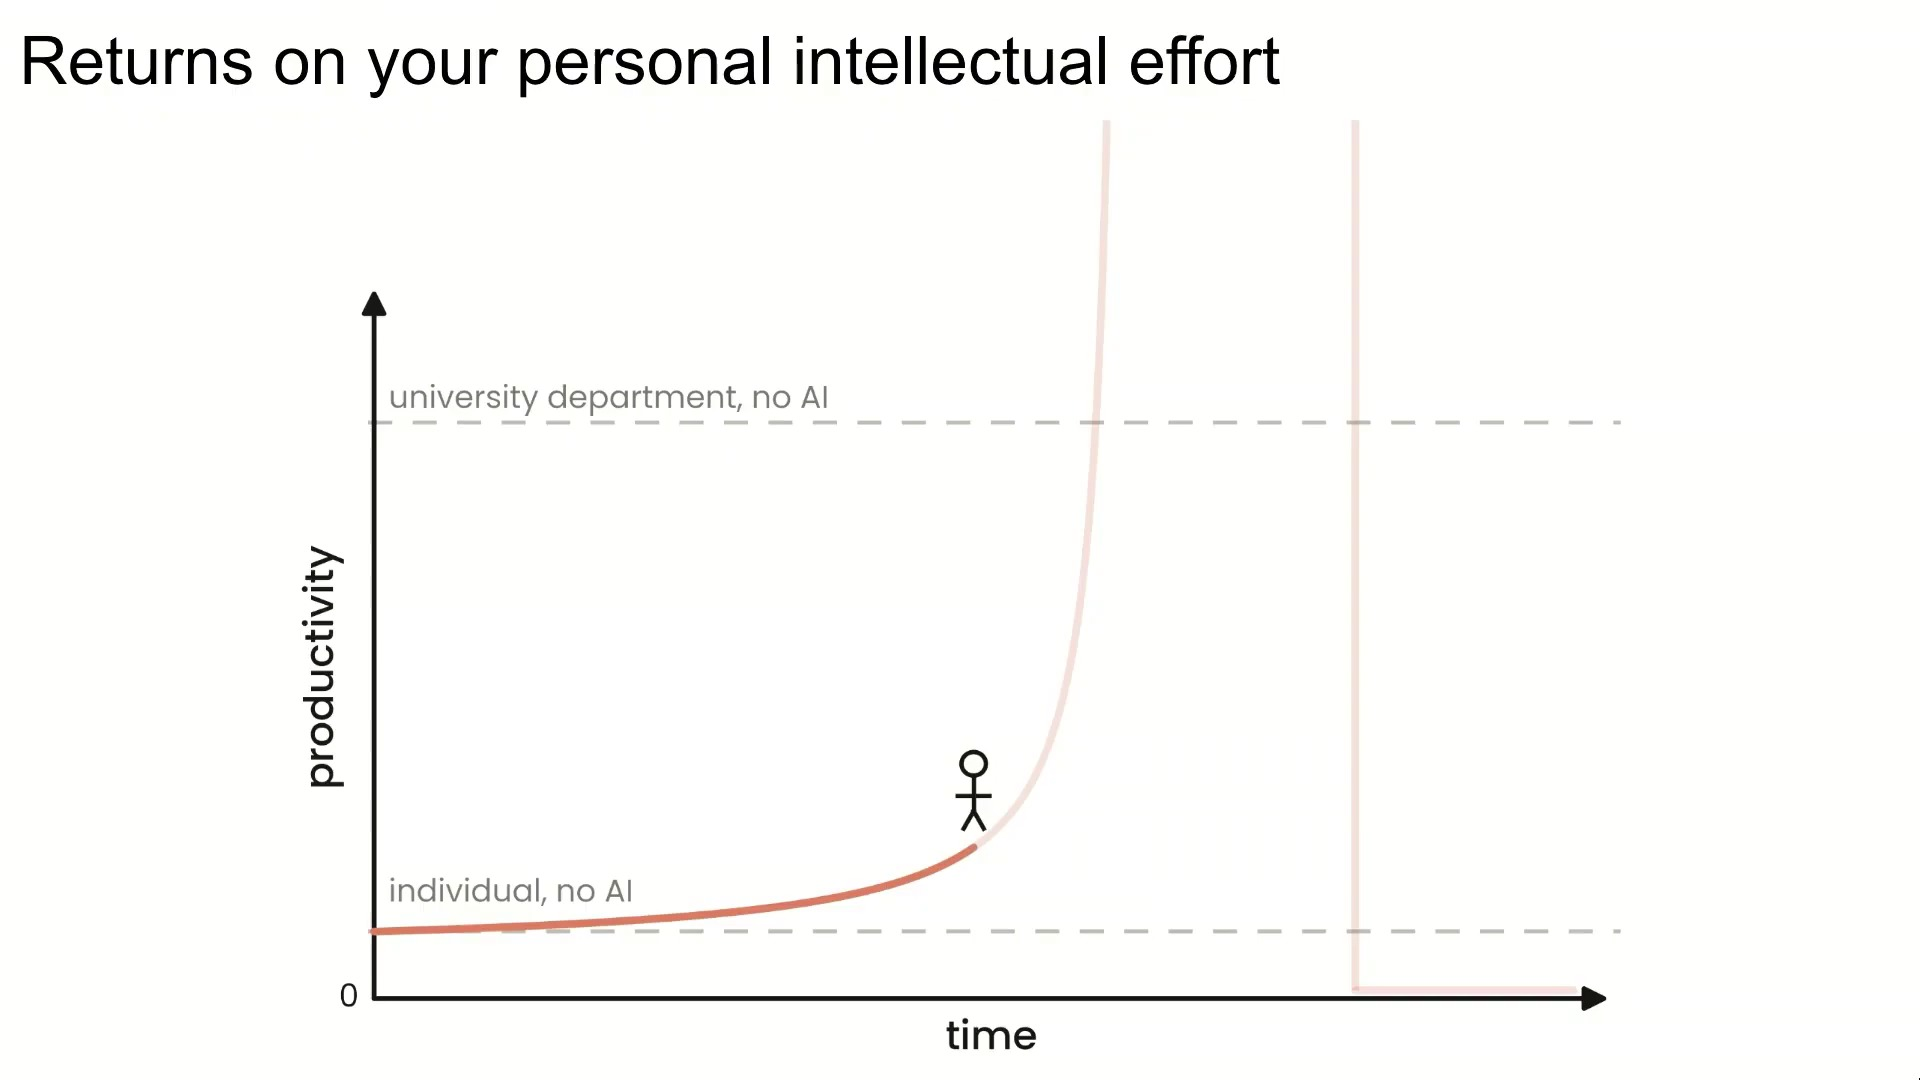
\includegraphics[width=0.92\textwidth]{figures/fig_18_intellectual_returns_curve.jpg}
\caption{个人智力投入回报率（Productivity vs.\ Time）的中期演化曲线：在 AI 工具加持下，单人科研生产力正从“无 AI 个人”快速跃升并超越“无 AI 的整个大学科系”，在全面认知自动化导致曲线归零前形成一段近乎垂直的黄金窗口期\vtag}
\end{figure}
\srcnote{00:31:55--00:32:39}

为了说明为什么“就是现在”至关重要，讲者绘制了上图的“个人智力投入回报曲线（Returns on your personal intellectual effort）”。图中包含两条水平虚线基准：下方虚线代表“没有 AI 时的单个研究者生产力（individual, no AI）”，上方虚线代表“没有 AI 时一所大学整整一个学系（university department, no AI）的总生产力”。随着 AI 工具的引入，单人生产力曲线（实心红线，小人所站位置）已经开始加速上扬；再往前走一小段（半透明粉色曲线），一名善于驾驭成百上千个 AI 科研 Agent 的独立研究者，其单人学术产出就将一举超越过去的整个大学科系，并冲向近乎垂直的渐近线——\textbf{这是人类智力史上前所未有的“超级个体黄金窗口期”}。然而，当曲线越过奇点、AI 完全无需人类提供高层直觉与品味指导时，人类个人智力投入的边际生产力将沿着右侧垂直线骤然跌回零点（$0$）。我们正站在这座陡峰起跳的脚下。

\subsection{本章小结}
本章通过 Epoch AI 的 2030 年算力瓶颈测算（即便受限于电力，训练算力仍将扩张 10,000 倍）证明了当下仍处指数极早期，剖析了 SMTP 协议、HeLa 细胞、Linux、四乙基铅与同行评审等九大历史案例的路径依赖机制，明确了研究者通过选题、命名框架与架构取向塑造 AI 技术树的五个支点，并揭示了单人科研生产力从超越整个大学科系到最终归零的黄金窗口曲线。

\clearpage
\section{六大高价值科研方向与深度问答交锋}

在报告的最后一部分，Sohl-Dickstein 结合前述四条准则与历史杠杆视角，向在场的青年学者具体推荐了他个人最为看好的\textbf{六大项目领域（Some project areas I like）}，并在随后的近 10 分钟里与听众展开了坦诚深入的问答探讨。

\subsection{讲者力荐的六大高杠杆研究与实践方向}

\begin{figure}[H]
\centering
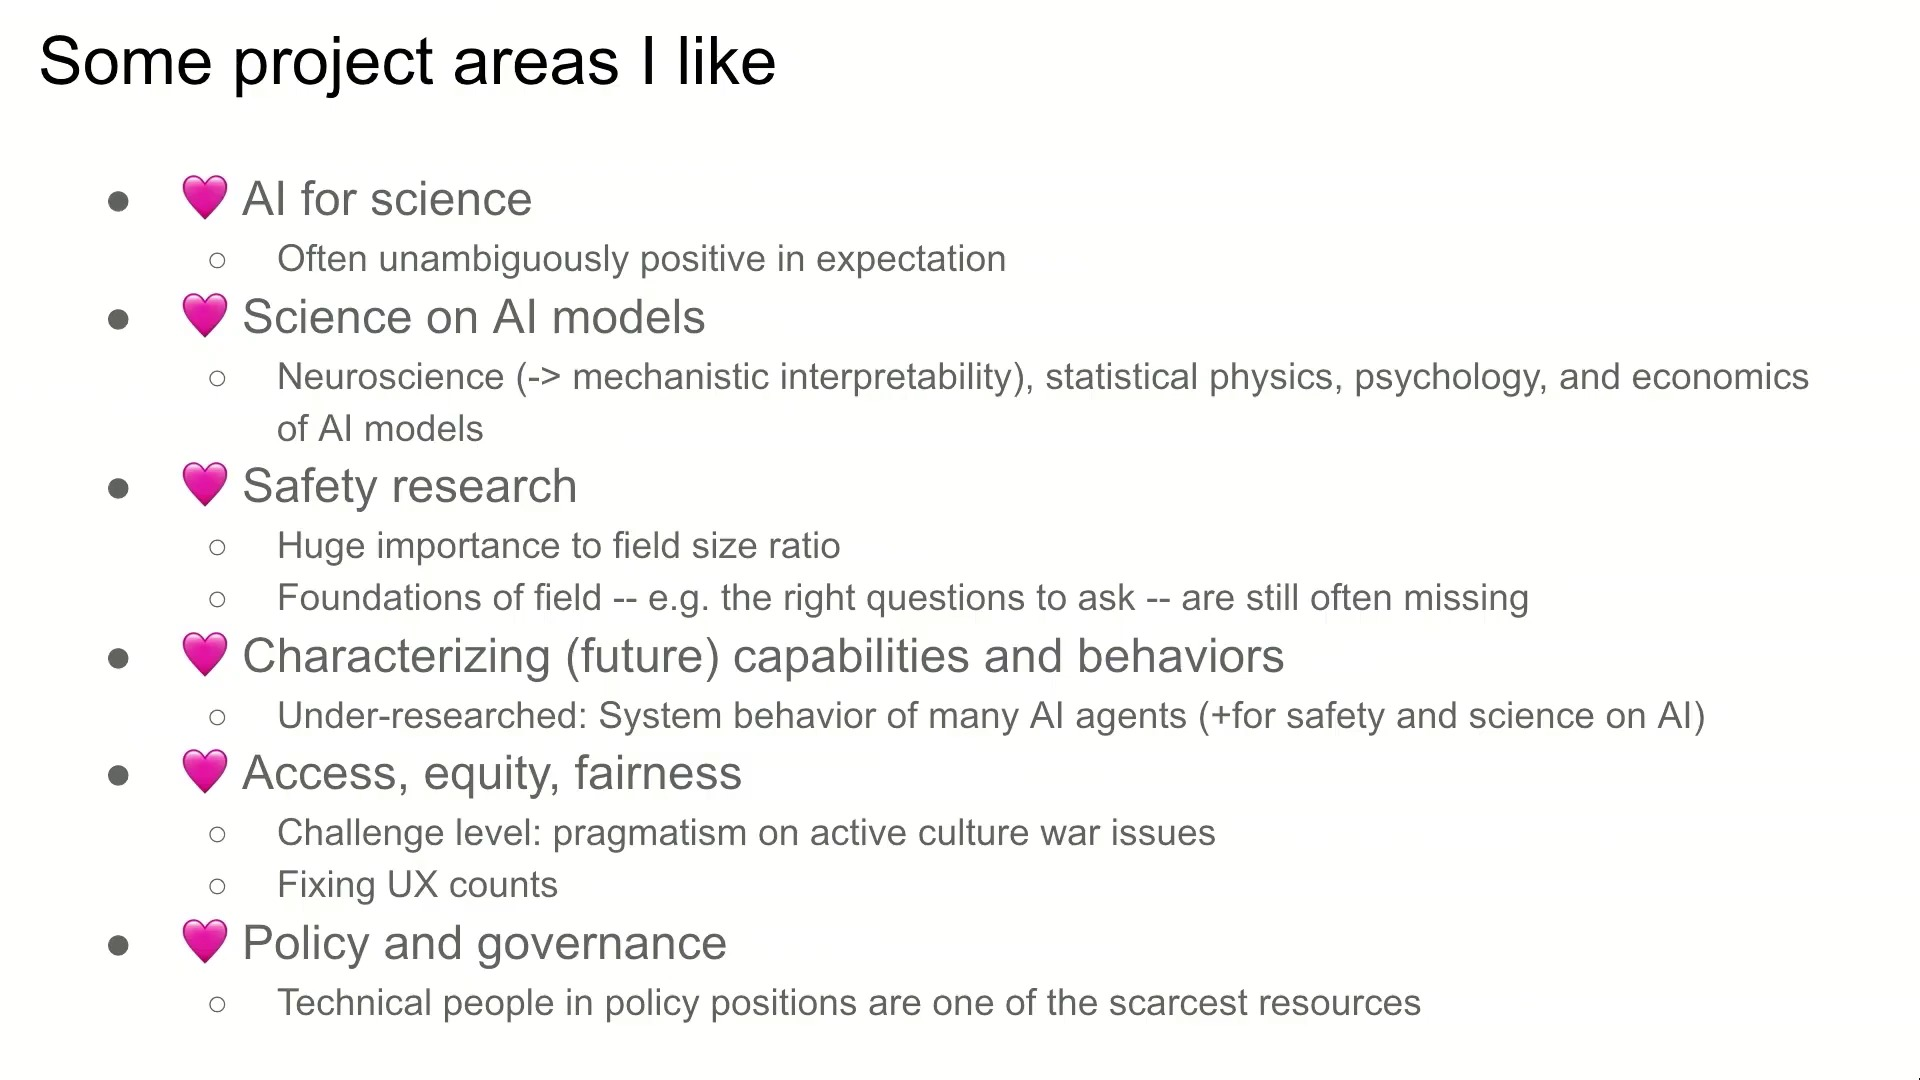
\includegraphics[width=0.92\textwidth]{figures/fig_19_project_areas.jpg}
\caption{Jascha Sohl-Dickstein 重点推荐的六大高价值研究与治理领域：科学智能（AI for Science）、以科学方法研究 AI 模型、安全研究、表征未来能力与多智能体系统行为、公平可及与 UX 改进，以及技术政策与治理\vtag}
\end{figure}
\srcnote{00:32:39--00:34:35}

围绕上图的六颗爱心条目，讲者逐一剖析了每个方向的独特价值与切入点：

\begin{table}[H]
\centering
\small
\caption{讲者推荐的六大高价值研究与实践领域全景对比}
\begin{tabular}{p{3.2cm}p{4.8cm}p{5.6cm}}
\toprule
\textbf{研究/实践领域} & \textbf{核心定位与稀缺性价值} & \textbf{具体切入课题与实操注意要点} \\
\midrule
1.\ AI for Science\newline（科学智能） & 期望社会收益几乎毫无争议地为正（Unambiguously positive in expectation），能直接加速生物医药、材料与物理发现 & 必须严格执行“特征时间尺度判据”：不要花两年手工微调一个明年就会被通用大模型零样本击败的窄领域小模型，而应构建高质量科学评测、实验闭环接口与形式化环境 \\
2.\ Science on AI Models\newline（对 AI 模型做科学） & 将深度神经网络视为自然界新出现的复杂系统客体，用成熟自然科学范式揭示其内部机理 & 四大交叉分支：\textbf{神经科学}（即机制可解释性 Mechanistic Interpretability）、\textbf{统计物理}（标度律与相变动力学）、\textbf{心理学}（认知偏差与行为测度）、\textbf{AI 经济学} \\
3.\ Safety Research\newline（AI 安全研究） & 重要性与当前从业人员规模之比（Importance to field size ratio）高得惊人 & 该领域的学科地基（Foundations of field）——甚至连“究竟应该提出哪些正确的科学问题”——目前仍是空白，早期奠基性工作具有极高的轨迹偏转杠杆 \\
4.\ Characterizing (Future) Capabilities \& Behaviors & 预判并表征下一代模型的能力边界与涌现行为，同时服务于 AI 安全与 AI 科学 & 讲者特别点出当前严重研究不足的蓝海：\textbf{由大量 AI 智能体组成的系统行为（System behavior of many AI agents）}，如多 Agent 生态的宏观博弈与涌现失控 \\
5.\ Access, Equity, Fairness\newline（可及性、公平与普惠） & 决定技术红利是由少数精英独占还是惠及全球普通人 & 挑战在于如何在激烈的文化战争议题（Culture war issues）中保持务实（Pragmatism）。讲者强调：\textbf{“改进用户体验也算数（Fixing UX counts）”}——消除使用门槛本身就是重大的公平贡献 \\
6.\ Policy and Governance\newline（政策与治理） & \textbf{“身处政策制定岗位的技术人才是目前全世界最稀缺的资源之一”} & 政府与立法机构迫切需要真正懂大模型训练、评测与安全机理的学者参与规则设计；这也是高校学者拥有天然中立公信力比较优势的核心舞台 \\
\bottomrule
\end{tabular}
\end{table}

\subsection{尾声深度问答：对齐失控、评审危机、多智能体博弈与“写作即思考”}

在报告最后的开放问答环节（对应视频 \texttt{00:34:35--00:44:34}），现场听众就 AI 安全失控的具体形态、学术同行评审的崩溃风险、高校的生存定位以及年轻学者的思维训练提出了五个尖锐问题：

\begin{importantbox}{尾声深度问答全记录（00:34:35--00:44:34）}
\begin{enumerate}
    \item \textbf{问：过度强调安全护栏是否会扼杀基础科学探索？你真正担心的对齐失败（Alignment Failure）究竟长什么样？}
    
    \textbf{Sohl-Dickstein 答}：我不认为合理的对齐研究是在给科学套枷锁，恰恰相反，它是确保人类能够安全抵达“戴森云时代”的前提。至于具体的失败形态，除了经典的“曲别针最大化器（Paperclip Maximizer，即模型为了单一代理目标而不择手段耗尽地球资源）”式极端失控外，我同样高度警惕一种更隐蔽、渐进的失控——例如由人类反馈强化学习（RLHF）过度优化导致的\textbf{病态讨好与操控（Sycophancy / Manipulation）}，或者全球关键基础设施在不知不觉中完全移交给人类已无法理解、无法关停的耦合智能体网络，最终导致人类集体丧失自主权。

    \item \textbf{问：当所有人都能用 AI 在几小时内生成看似完美的论文，传统同行评审（Peer Review）系统是否会因垃圾论文泛滥而彻底瘫痪？}
    
    \textbf{Sohl-Dickstein 答}：正如前面历史列表所指出的，现代匿名同行评审制度本身也不过是二战后才建立起来的年轻制度，绝非不可更改的金科玉律。当生成一篇形式合规论文的边际成本趋近于零时，依赖人工逐字审阅文本的旧认证体系必然面临信噪比危机。未来的科学共同体必须演化出新的过滤与验证机制——例如强制要求可复现的代码/实验沙箱验证、形式化证明检查（如 Lean），或者借助经过严格校准的 AI 审稿辅助与新型学术声誉网络。

    \item \textbf{问：你为什么特别强调“多智能体系统行为（System behavior of many AI agents）”是一个被严重低估的方向？}
    
    \textbf{Sohl-Dickstein 答}：目前绝大多数评测与对齐工作都聚焦于“单个模型与单个用户的对话（Single-model, single-user）”。然而在未来几年内，真实世界将充满数以亿计彼此调用、彼此谈判、共同争夺算力与经济资源的自主 Agent。在统计物理与经济学中我们熟知，即便每一个微观个体本身都是温顺且局部理性的，当大量个体耦合交互时，系统层面依然可能自发涌现出闪电崩盘、公地悲剧、多方囚徒困境乃至恶性军备竞赛。我们对 AI 群体的宏观相变与社会动力学几乎一无所知。

    \item \textbf{问：高校既没有工业界万卡集群的算力，也开不出硅谷实验室的薪酬，大学在未来 1--5 年还有什么比较优势（Comparative Advantage）？}
    
    \textbf{Sohl-Dickstein 答}：如果高校课题组试图去和前沿工业实验室比拼“从头预训练一个更大的通用基础模型”，那确实毫无胜算。但高校拥有一项工业界永远无法凭空买到的宝贵资产——\textbf{制度公信力与利益超脱性（Trust and Credibility）}。当 Anthropic 或 OpenAI 向政府和公众宣称“我们的模型很安全、应该这样监管”时，外界天然会怀疑其中掺杂了商业利益或监管俘获；而一位没有任何商业利益捆绑的斯坦福或哈佛独立学者所做出的第三方审计、多智能体风险测度、经济学冲击评估与治理方案，在立法者与社会公众眼中具有不可替代的分量。

    \item \textbf{问：你刚才提到“绝不要让 AI 替你写论文初稿”，能否展开谈谈？在 AI 时代我们该如何培养年轻研究者的思考能力？}
    
    \textbf{Sohl-Dickstein 答}：我坚信\textbf{“写作即思考（Writing is thinking）”}。很多时候，在你动笔把一个模糊的科学构想写成结构严密的自然段之前，你以为自己已经想明白了，但其实你的逻辑链条里到处都是跳跃和漏洞。正是亲手遣词造句、推导公式、组织论证的痛苦过程，逼迫你的大脑完成了最深层的概念整合与自我纠错。如果一开始就让 Claude 替你生成流畅华丽的初稿，你的大脑就会直接跳过这一核心锻造环节，沦为被动的文字审阅者。因此，最理想的工作流是：\textbf{由你自己亲手写出哪怕粗糙但逻辑真实的初稿，然后再调用大模型强大的批判与润色能力来迭代打磨}。
\end{enumerate}
\end{importantbox}

\subsection{本章小结}
本章系统拆解了讲者推荐的六大高杠杆方向（科学智能、对 AI 模型做跨学科科学、安全地基研究、多智能体系统行为表征、务实的公平可及与 UX 改进、技术人才投身政策治理），并通过尾声五大问答厘清了对齐失控的双重形态、同行评审制度的演化方向、多 Agent 宏观博弈风险、高校在公信力与独立审计上的核心比较优势，以及坚守“写作即思考”的认知训练底线。

\clearpage
\section{总结与延伸}

\subsection{演讲核心逻辑闭环回顾}

纵观整场 45 分钟的报告，Jascha Sohl-Dickstein 以极其凝练的科学家视角完成了一次从“宏观历史定位”到“微观个人行动”的严密推演：
\begin{enumerate}
    \item \textbf{历史坐标与实证底座}：始于 1950 年的“人类世”正迎来其技术加速的顶点。2010--2025 年间前沿训练算力以年均 $4.7\times$ 激增 1000 万倍并逼近人脑毕生总算力（$\sim 10^{12}\text{ petaFLOP}$），METR 软件工程 50\%（及 80\%、90\%）可靠完成跨度从 4 秒跃迁至 10 小时，开放 Erdős 数学猜想在 7 个月内被攻克 56 题（27 题全自主）。三条对数直线共同支撑起旧金山前沿实验室 \textbf{1--5 年实现 AGI}（长线派亦仅 10--30 年）的内部共识，并推动全球政商与媒体奥弗顿之窗在 2025 年发生剧烈迁移。
    \item \textbf{个人窗口期的四项行动准则}：面对仅剩 1--5 年的传统智力贡献窗口，研究者必须：（a）确保项目周期短于指数特征尺度（$\tau_{\text{project}} < \tau_{\text{exp}}$），遵循《苦涩的教训》借力规模扩张；（b）克服“无马马车”的初期别扭感，将大模型深度融入构思、审稿反馈（坚持手写初稿）、编码与一次性交互看板，发挥做 PI 与写 Prompt 的任务拆解同构性；（c）消除“信 3 年 AGI 却走 10 年传统教职”的认知失调，在高基线颠覆风险下果断追求最高上限；（d）放弃瞬态刷榜，选择能偏转长期轨迹（Shift the trajectory）的课题。
    \item \textbf{早期介入的万倍杠杆与六大落地方向}：Epoch AI 测算表明 2030 年训练算力即便受最严苛的电力约束仍将比现在大 10,000 倍，证明当下仍处指数极早期。如同 1980 年制定 SMTP 协议或二战后确立同行评审制度一样，今天研究者在 AI for Science、AI 模型科学（机制可解释性、统计物理、心理学、经济学）、安全地基、多智能体系统行为、务实 UX 普惠以及技术治理上的每一个微小抉择，都将被未来的指数扩张放大为决定人类后人类世命运的长期路径依赖。
\end{enumerate}

\subsection{综合评述与批判性延伸}

站在读者的视角审视这场报告，无论你是否完全认同旧金山实验室“1--5 年内实现全面 AGI”的激进时间线，Sohl-Dickstein 提出的分析框架都具有极强的\textbf{策略鲁棒性（Strategic Robustness）}：
\begin{itemize}
    \item \textbf{即使 AGI 需要 10--20 年才会全面成熟}，那些能够跨数量级延长任务跨度的编程与推理模型也已经在当下彻底改变了科研生产函数。遵循“缩短反馈周期、避开纯靠算力就能顺手解决的修补性工作、用一次性看板加速探索、坚守亲手写初稿的深度思考”这四条原则，依然能让一位青年学者在未来五年的学术竞争中获得远超同侪的学术生产力。
    \item \textbf{从“瞬态增量”转向“轨迹偏转”的价值重估}：当前机器学习与各交叉学科顶会中充斥着大量寿命不足三个月的微小刷榜论文。讲者以历史案例（SMTP vs.\ 即时通讯割裂、HeLa 细胞共享、四乙基铅教训）敲响的警钟提醒我们：在技术形态尚未完全固化的窗口期，制定一套开源评测标准、揭示一类多智能体博弈失灵机制、构建一个降低普通人使用门槛的交互范式，或是以独立学者身份撰写一份严谨的技术治理报告，其长远历史权重远胜于在拥挤不堪的存量赛道上把某个指标提前几周推高半个百分点。
\end{itemize}

%% --- 正文内容结束 --- %%

\end{document}
